\documentclass[degree=bachelor,tocarialchapter]{thuthesis}
% 选项
%   degree=[bachelor|master|doctor|postdoctor], % 必选,学位类型
%   language=[chinese|english], % 可选(默认:chinese),论文的主要语言
%   secret,                % 可选(默认:关闭),是否有密级
%   tocarialchapter,       % 可选(默认:关闭),章目录中使用黑体(这项表示同时打开下面两项)
%   tocarialchapterentry,  % 可选(默认:关闭),单独控制章标题在目录中使用黑体
%   tocarialchapterpage,   % 可选(默认:关闭),单独控制章页码在目录中使用黑体

% 所有其它可能用到的包都统一放到这里了,可以根据自己的实际添加或者删除。
\usepackage{thuthesis}
\usepackage{listings}
\usepackage{color}

\definecolor{dkgreen}{rgb}{0,0.6,0}
\definecolor{gray}{rgb}{0.5,0.5,0.5}
\definecolor{mauve}{rgb}{0.58,0,0.82}

\lstset{frame=tb,
  language=Python,
  aboveskip=3mm,
  belowskip=3mm,
  showstringspaces=false,
  columns=flexible,
  basicstyle={\small\ttfamily},
  numbers=none,
  numberstyle=\tiny\color{gray},
  keywordstyle=\color{blue},
  commentstyle=\color{dkgreen},
  stringstyle=\color{mauve},
  breaklines=true,
  breakatwhitespace=true,
  tabsize=3
}

\usepackage[linesnumbered,lined,ruled,vlined,commentsnumbered]{algorithm2e}
\usepackage{amsmath}
\DeclareMathOperator*{\argmax}{arg\,max}
\DeclareMathOperator*{\argmin}{arg\,min}
\usepackage{longtable}
% 定义所有的图片文件在 figures 子目录下
\graphicspath{{figures/}}

% 可以在这里修改配置文件中的定义。导言区可以使用中文。
% \def\myname{薛瑞尼}

\begin{document}

%%% 封面部分
\frontmatter
\thusetup{
  %******************************
  % 注意:
  %   1. 配置里面不要出现空行
  %   2. 不需要的配置信息可以删除
  %******************************
  %
  %=====
  % 秘级
  %=====
  secretlevel={秘密},
  secretyear={10},
  %
  %=========
  % 中文信息
  %=========
  ctitle={清华大学学位论文},
  cdegree={工学学士},
  cdepartment={土木工程系},
  cmajor={土木工程},
  cauthor={谭泽人},
  csupervisor={李瑞敏教授},
  cassosupervisor={陈文光教授}, % 副指导老师
  ccosupervisor={某某某教授}, % 联合指导老师
  % 日期自动使用当前时间,若需指定按如下方式修改:
  % cdate={超新星纪元},
  %
  % 博士后专有部分
  catalognumber     = {分类号},  % 可以留空
  udc               = {UDC},  % 可以留空
  id                = {编号},  % 可以留空: id={},
  cfirstdiscipline  = {计算机科学与技术},  % 流动站(一级学科)名称
  cseconddiscipline = {系统结构},  % 专 业(二级学科)名称
  postdoctordate    = {2009 年 7 月——2011 年 7 月},  % 工作完成日期
  postdocstartdate  = {2009 年 7 月 1 日},  % 研究工作起始时间
  postdocenddate    = {2011 年 7 月 1 日},  % 研究工作期满时间
  %
  %=========
  % 英文信息
  %=========
  etitle={An Introduction to \LaTeX{} Thesis Template of Tsinghua University v\version},
  % 这块比较复杂,需要分情况讨论:
  % 1. 学术型硕士
  %    edegree:必须为Master of Arts或Master of Science(注意大小写)
  %             “哲学、文学、历史学、法学、教育学、艺术学门类,公共管理学科
  %              填写Master of Arts,其它填写Master of Science”
  %    emajor:“获得一级学科授权的学科填写一级学科名称,其它填写二级学科名称”
  % 2. 专业型硕士
  %    edegree:“填写专业学位英文名称全称”
  %    emajor:“工程硕士填写工程领域,其它专业学位不填写此项”
  % 3. 学术型博士
  %    edegree:Doctor of Philosophy(注意大小写)
  %    emajor:“获得一级学科授权的学科填写一级学科名称,其它填写二级学科名称”
  % 4. 专业型博士
  %    edegree:“填写专业学位英文名称全称”
  %    emajor:不填写此项
  edegree={Doctor of Engineering},
  emajor={Computer Science and Technology},
  eauthor={Xue Ruini},
  esupervisor={Professor Zheng Weimin},
  eassosupervisor={Chen Wenguang},
  % 日期自动生成,若需指定按如下方式修改:
  % edate={December, 2005}
  %
  % 关键词用“英文逗号”分割
  ckeywords={TeX, LaTeX, CJK, 模板, 论文},
  ekeywords={TeX, LaTeX, CJK, template, thesis}
}

% 定义中英文摘要和关键字
\begin{cabstract}
  论文的摘要是对论文研究内容和成果的高度概括。摘要应对论文所研究的问题及其研究目
  的进行描述,对研究方法和过程进行简单介绍,对研究成果和所得结论进行概括。摘要应
  具有独立性和自明性,其内容应包含与论文全文同等量的主要信息。使读者即使不阅读全
  文,通过摘要就能了解论文的总体内容和主要成果。

  论文摘要的书写应力求精确、简明。切忌写成对论文书写内容进行提要的形式,尤其要避
  免“第 1 章……;第 2 章……;……”这种或类似的陈述方式。

  本文介绍清华大学论文模板 \thuthesis{} 的使用方法。本模板符合学校的本科、硕士、
  博士论文格式要求。

  本文的创新点主要有:
  \begin{itemize}
    \item 用例子来解释模板的使用方法;
    \item 用废话来填充无关紧要的部分;
    \item 一边学习摸索一边编写新代码。
  \end{itemize}

  关键词是为了文献标引工作、用以表示全文主要内容信息的单词或术语。关键词不超过 5
  个,每个关键词中间用分号分隔。(模板作者注:关键词分隔符不用考虑,模板会自动处
  理。英文关键词同理。)
\end{cabstract}

% 如果习惯关键字跟在摘要文字后面,可以用直接命令来设置,如下:
% \ckeywords{\TeX, \LaTeX, CJK, 模板, 论文}

\begin{eabstract}
   An abstract of a dissertation is a summary and extraction of research work
   and contributions. Included in an abstract should be description of research
   topic and research objective, brief introduction to methodology and research
   process, and summarization of conclusion and contributions of the
   research. An abstract should be characterized by independence and clarity and
   carry identical information with the dissertation. It should be such that the
   general idea and major contributions of the dissertation are conveyed without
   reading the dissertation.

   An abstract should be concise and to the point. It is a misunderstanding to
   make an abstract an outline of the dissertation and words ``the first
   chapter'', ``the second chapter'' and the like should be avoided in the
   abstract.

   Key words are terms used in a dissertation for indexing, reflecting core
   information of the dissertation. An abstract may contain a maximum of 5 key
   words, with semi-colons used in between to separate one another.
\end{eabstract}

% \ekeywords{\TeX, \LaTeX, CJK, template, thesis}

% 如果使用授权说明扫描页,将可选参数中指定为扫描得到的 PDF 文件名,例如:
% \makecover[scan-auth.pdf]
\makecover

%% 目录
\tableofcontents

%% 符号对照表
\begin{denotation}[3cm]
\item[HPC] 高性能计算 (High Performance Computing)
\item[cluster] 集群
\item[Itanium] 安腾
\item[SMP] 对称多处理
\item[API] 应用程序编程接口
\item[PI] 聚酰亚胺
\item[MPI] 聚酰亚胺模型化合物,N-苯基邻苯酰亚胺
\item[PBI] 聚苯并咪唑
\item[MPBI] 聚苯并咪唑模型化合物,N-苯基苯并咪唑
\item[PY] 聚吡咙
\item[PMDA-BDA]	均苯四酸二酐与联苯四胺合成的聚吡咙薄膜
\item[$\Delta G$] 活化自由能 (Activation Free Energy)
\item[$\chi$] 传输系数 (Transmission Coefficient)
\item[$E$] 能量
\item[$m$] 质量
\item[$c$] 光速
\item[$P$] 概率
\item[$T$] 时间
\item[$v$] 速度
\item[劝学] 君子曰:学不可以已。青,取之于蓝,而青于蓝;冰,水为之,而寒于水。木
  直中绳。輮以为轮,其曲中规。虽有槁暴,不复挺者,輮使之然也。故木受绳则直,金就
  砺则利,君子博学而日参省乎己,则知明而行无过矣。吾尝终日而思矣,不如须臾之所学
  也;吾尝跂而望矣,不如登高之博见也。登高而招,臂非加长也,而见者远;顺风而呼,
  声非加疾也,而闻者彰。假舆马者,非利足也,而致千里;假舟楫者,非能水也,而绝江
  河,君子生非异也,善假于物也。积土成山,风雨兴焉;积水成渊,蛟龙生焉;积善成德,
  而神明自得,圣心备焉。故不积跬步,无以至千里;不积小流,无以成江海。骐骥一跃,
  不能十步;驽马十驾,功在不舍。锲而舍之,朽木不折;锲而不舍,金石可镂。蚓无爪牙
  之利,筋骨之强,上食埃土,下饮黄泉,用心一也。蟹六跪而二螯,非蛇鳝之穴无可寄托
  者,用心躁也。—— 荀况
\end{denotation}



% % 也可以使用 nomencl 宏包:

% \printnomenclature[3cm]

% \nomenclature{HPC}{高性能计算 (High Performance Computing)}
% \nomenclature{cluster}{集群}
% \nomenclature{Itanium}{安腾}
% \nomenclature{SMP}{对称多处理}
% \nomenclature{API}{应用程序编程接口}
% \nomenclature{PI}{聚酰亚胺}
% \nomenclature{MPI}{聚酰亚胺模型化合物,N-苯基邻苯酰亚胺}
% \nomenclature{PBI}{聚苯并咪唑}
% \nomenclature{MPBI}{聚苯并咪唑模型化合物,N-苯基苯并咪唑}
% \nomenclature{PY}{聚吡咙}
% \nomenclature{PMDA-BDA}{均苯四酸二酐与联苯四胺合成的聚吡咙薄膜}
% \nomenclature{$\Delta G$}{活化自由能 (Activation Free Energy)}
% \nomenclature{$\chi$}{传输系数 (Transmission Coefficient)}
% \nomenclature{$E$}{能量}
% \nomenclature{$m$}{质量}
% \nomenclature{$c$}{光速}
% \nomenclature{$P$}{概率}
% \nomenclature{$T$}{时间}
% \nomenclature{$v$}{速度}



%%% 正文部分
\mainmatter
\chapter{文献综述}
\label{chap:liter}
\section{背景介绍}
近些年来,随着信息技术以及其他领域的发展,逐渐有两个趋势变得明显,并且将极大的影响人们的生活。
\par
一方面,电子,自动化,计算机等技术的提高,使得无人驾驶技术逐渐受到关注。美国汽车工程师协会奖自动驾驶技术被分为六个层级,从最低级的L0级,即无自动化驾驶,人类全权驾驶,到最高级L5,即完全自动化技术,汽车可以在任何的道路和环境条件下,完成所有的驾驶操作,只在可能的情况下会让人类接管。目前的技术水平已经达到了L3级,即在人类提供一定的应答的情况下驾驶。自动驾驶车辆作为一种新型的交通工具,它可以极大地提高出行的安全性和效率\cite{lee2019autonomous}。但是,目前已有的研究中,考虑自动驾驶车辆情境下的交通行为还较少,对于这样会在很大程度上改变交通出行行为的工具,还需要很多的研究者进行研究。
\par
另一方面,“共享经济”的改变逐渐进入人们的视野。共享单车已经从几年前的不见踪影,到现在的俯拾即是。以ofo,Moobike等为首的一众公司将共享单车推进了人们的生活。Airbnb提供了将人们房子的空闲房间共享的平台,使得“酒店”、“旅馆”等住宿形式之外,衍生出一种更加低成本的,低门槛的、便捷的住宿形式。原本私人的房间也称为陌生人之间可以共享的物品。Uber、Lyft、滴滴等公司推出了出行的共享服务。不同的人可以进行拼车,共用同一辆汽车。这样的经济模式不仅方便了人们的生活,而且带来了许多新兴的经济生产力,实现了多方面的共赢。对于交通领域的学者来说,需要紧跟时代脚步,对新兴出现的ride-sharing模式进行研究,为平台和系统的高效率运行提供支持。
\par
本文即在考虑这样的两种趋势下,希望对城市中出现和可能出现的交通模式,通过算法的求解,找到较为优的解,提高系统的运行效率,减少交通拥堵,减少尾气排放,减少路面上的车。更准确的说,本文想研究的问题,有以下三个:
\begin{enumerate}
\item 在假设全部的车辆都为自动驾驶的情形下,每个选择乘坐自动驾驶车辆出行的乘客都通过中心平台申请自己的出行需求,包括出发的时间,出发的地点,目的地的位置,所能接受的最晚到达时间。我们希望设计一种机制和算法,将所有的乘客出行通过它们的时间和空间关系,串联起来,串联在一起的出行分配给同一辆车接送,我们的目标是希望找到最少的车辆服务所有的出行。这我们将在第~\ref{chap:num}~章进行详细的讨论。
\item 在允许不同的出行之间进行合乘的情形下,每个可以接受合乘的乘客通过中心平台向平台发送出行请求,输入包括出发的时间,出发的地点,目的地的位置,所能接受的到达的最晚时间。我们考虑的合乘为较简单情形的合乘——两个出行进行合乘。我们根据合乘后的出行的数据进行串联,每一条串联的路上的出行都被分配给同一辆车进行接送,我们希望减少路面上的车辆,所以目标为以最少的车辆服务所有的出行需求。这我们将在第~\ref{chap:share}~章进行详细的讨论。
\item 在考虑了两个出行的合乘之后,我们进一步考虑多个出行的合乘,并且考虑车辆的容量,我们希望研究出行之间的组合,即合乘的机制和方法,以及将合乘后的出行分配给车辆的算法。由于问题的难度很大,我们只研究在很短时间内的出行组合以及出行和车辆的匹配。我们通过数学建模,提出解决问题的最优解的算法,并通过实验讨论算法的效率。这一部分我们将在第~\ref{chap:ridesharing}~章详细讨论。
\end{enumerate}

\section{前人研究}

\chapter{寻找车座数不同情形下所需最少车辆}
\label{chap:num}

在之前的讨论中,我们假设每一个出行的人数都为1。但是实际上,不同的出行可能会有不同的出行人数,即,一辆车可能承载了超过1人,可能承载了2人,3人,4人。根据实际的出行数据我们可以得到,平均每辆车的乘客数为1.3人,可以想见,车辆的利用效率时比较低的。现在的私人汽车,出租车等出了司机外,还可乘载4人,现在的汽车的座位利用情况较差。同时,这样的汽车体积浪费也在很大程度上加剧了交通拥堵。
\par
由此我们就可以想到,如果有大量的两座车,代替现在的四座车,车辆在路上占有的道路面积就会减少,道路中就可以容纳更多的车辆。相应地,交通拥堵就会减少,尾气排放就会减少,环境污染就得到了减缓。所以在考虑乘客数量的情形下,我们可以进一步地得到所需最少的相应座数的车辆数,进而得到所需要的总共的车辆数。

\section{数据来源}
经过数据预处理后的数据分为两个部分。
\par
第一部分的数据为廊坊市一天中的所有出行数据,每一条数据中包含出行的索引,出行的出发时间和到达时间,出行的出发地点和到达地点,以及乘客数量,具体的数据解释见下表~\ref{tab:triplist}。
\begin{table}
    \centering
    \caption{出行数据的具体解释}
    \label{tab:triplist}
  \begin{tabular}{|c|p{10cm}|}
    \hline
    数据项 & 具体解释\\
    \hline \hline 
    tripRowid & 出行数据的索引,但是不是按照时间顺序排列的\\
    \hline 
    oTime & 出行的出发时间,将时间转化为秒,一天中最小的为0秒,最大的为86400秒\\
    \hline 
    dTime & 出行的到达时间,将时间转化为秒,一天中最小的为0秒,最大的为86400秒\\
    \hline 
    oInter & 出行的出发地点,将地点转化为交叉口编号,在之后的计算中出行的地理位置信息,都按照交叉口的地理信息计算\\
    \hline 
    dInter & 出行的到达地点,将地点转化为交叉口编号,在之后的计算中出行的地理位置信息,都按照交叉口的地理信息计算\\
    \hline 
    numPassen & 出行中乘客的数量,最少为1人,最多为4人\\
    \hline 
  \end{tabular}
\end{table}

\par
第二部分的数据为廊坊市所有交叉路口两两之间的汽车行驶时间,廊坊市共78个交叉路口,我们根据百度地图API的结果,得到每两个交叉路口之间的行驶时间,所以我们得到了一个$78\times 78$的矩阵$Dis$,该数据表中的数据信息如表~\ref{tab:odtime}~所示。

\begin{table}
  \centering
  \caption{交叉路口之间的出行时间}
  \label{tab:odtime}
  \begin{tabular}{|c|c|}
  \hline 
  数据项 & 具体解释\\
  \hline \hline 
  o & 出发交叉口的编号\\
  \hline 
  d & 到达交叉口的编号\\
  \hline 
  time & 根据百度地图API得到的从o到d的汽车行驶时间\\
  \hline 
  \end{tabular}
\end{table}

\section{匹配算法设计与分析}
这一部分,我们将介绍不同出行之间的匹配算法的设计与分析。
\subsection{算法设计思路}
由于本问题具有很强的图与网络的直观意义,所以下面我们选择使用图和网络的算法进行建模计算。
\par
按照前一部分我们对数据的解释,每一个出行,都包含五个数据项$(t^o, t^d, I^o, I^d, n_i)$,分别代表出行的出发时间,到达时间,出发交叉路口,到达交叉路口,乘客数量。
\par
每一个出行,我们都可以看成为时间和空间共同组成的空间上的一个节点,根据一定的判定条件,可以决定两个出行之间是否有边。由于两次出行之间存在天然的时间上的差异,所以所有形成的网络中的边都为有向边,另一方面,根据我们后面要提出的判别条件可以知道,只有当两个出行的时间之间满足一定的条件,才能够有边相连。在最终形成的网络中,两个出行之间有边,代表他们可能可以被同一辆车先后服务,最终它们是否可以被同一辆车在不同的时间服务,取决于最终算法的求解结果。
\par
两个出行之间可以有一条有向边相连,必须满足一定的条件。由于这里我们不考虑不同出行之间的合乘,则两个出行之间的出行时间需要满足一定关系,正式的数学表述如下:设$tr_i = (t_i^o, t_i^d, I_i^o, I_i^d, n_i), tr_j = (t_j^o, t_j^d, I_j^o, I_j^d, n_j)$,不妨设$t_i^o < t_j^o$,则若$t_i^d + travel(I_i^d, I_j^o) > t_j^o$,则两个出行所代表的节点之间没有边。
\par
除此之外,由于我们现在考虑了车座数的影响,我们这里设定有两种车座数的车,分别是2座车,4座车。并且,2座车只载有一个乘客或者两个乘客的出行,4座车只载有三个乘客或者四个乘客的出行。所以两个出行的乘客数之间也需要满足一定的关系:若$|n_i - n_j| > 1$,则两次出行之间没有有向边;否则,若$\max(n_i, n_j) = 3$并且$\min (n_i, n_j) = 2$,则它们之间也没有有向边;否则,若它们满足上述出行时间的关系,则它们之间有有向边相连。
\par
综上所述,我们可以将判断两个出行是否可能可以被同一辆车服务的算法写成如Alg.\ref{alg:islink}~所示的伪代码:

\begin{algorithm}[htbp]
\SetAlgoLined
\SetKwInOut{Input}{Input}\SetKwInOut{Output}{Output}
\caption{isLinkable($tr_i,tr_j$)}
\label{alg:islink}
\BlankLine
\uIf{$|n_i - n_j|>1$}{
  return False\;
}
\uElseIf{(max($n_i, n_j$)==3) and (min($n_i, n_j$)==2)}{
  return False\;
}
\uIf{$t_i^o > t_j^o$}{
  $tr_1 = tr_j$\;
  $tr_2 = tr_i$\;
}
\uElse{
  $tr_1 = tr_i$ \;
  $tr_2 = tr_j$ \;
}
\uIf{$t_1^d + travel(I_1^d, I_2^o) < t_2^o$}{
  return True\;
}
\uElse{
  return False\;
}
return False\;
\end{algorithm}

\subsection{算法时间复杂度分析}
从算法~\ref{alg:islink}~可以看出,算法中除了\texttt{travel$(I_1^d, I_2^o)$}之外,只有时间的大小比较,以及\texttt{if-else}语句的条件判断,所以容易知道,除了\texttt{travel$(I_1^d, I_2^o)$}之外,所有的语句的时间复杂度为$O(1)$。但是由于\texttt{travel$(I_1^d, I_2^o)$}是根据$Dis$计算得到,我们在得到了$Dis$这个$78\times 78$矩阵之后,进一步将其转变为Hash表,对于Hash表而言,从中查询一个元素的时间复杂度为$O(1)$。而在计算\texttt{travel$(I_1^d, I_2^o)$}时,我们即是查询$Dis(I_1^d, I_2^o)$,这样的一次计算的时间复杂度为$O(1)$,所以我们就可以得到算法~\ref{alg:islink}~的时间复杂度为$O(1)$。

\section{网络生成算法的设计与分析}
\subsection{算法设计}
在前一部分我们已经介绍了判断两个出行是否可以被同一辆车服务的算法,即网络中的两个节点是否可以有边相连的算法。这一部分,我们将介绍利用算法~\ref{alg:islink}~生成网络的算法。
\par
由于我们将每个出行视为网络中的一个节点,所以我们只需要对每两个节点判断它们之间是否可以有边相连即可。算法的伪代码如算法~\ref{alg:genegraph}:
\begin{algorithm}[htbp]
\SetAlgoLined
\SetKwInOut{Input}{Input}\SetKwInOut{Output}{Output}
\caption{generateGraph($Tr$)}
\label{alg:genegraph}
\BlankLine
初始化有向图网络$G \leftarrow \emptyset$\;
\For{$tr_i$ in $Tr$}{
  \tcp{$Tr(k:)$代表索引在$k$及以后的出行的集合;}
  \For{$tr_j$ in $Tr(i+1:)$}{
    \uIf{isLinkable($tr_i, tr_j$)}{
      \uIf{$t_i^o < t_j^o$}{
        $G\leftarrow G\cup \{(tr_i, tr_j)\}$\;
      }
      \uElse{
        $G\leftarrow G\cup \{(tr_j, tr_i)\}$\;
      }
    }
  }
}
return $G$\;
\end{algorithm}
\par
按照此算法生成网络的示意图如图~\ref{fig:net}~所示。
\begin{figure}
\centering
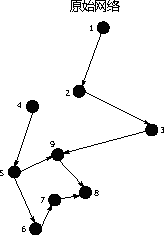
\includegraphics[width=5cm]{./figures/img/originalNetwork.pdf}
\caption{算法生成网络的示意图}
\label{fig:net}
\end{figure}
\subsection{算法时间复杂度分析}
从算法~\ref{alg:genegraph}~中可以看出,在循环内部的条件判断语句和对$N$的赋值语句的时间复杂度都为$O(1)$的,从前一部分的分析又知道\texttt{isLinkable($tr_i,tr_j$)}的时间复杂度为$O(1)$。对于$Tr$中的每一个出行$tr_i$,我们都将其与索引在$i$之后的所有出行$Tr(i+1:)$进行判断,设$m = |Tr|$,则总共判断了$\frac{m(m-1)}{2}$次,所以以上算法的时间复杂度为$O(\frac{m(m-1)}{2})$。由于想要得到完整的网络,我们必须对$Tr$中的所有出行组成的所有出行对进行分析,由于有$m$个出行数据,我们就必须进行至少$\frac{m(m-1)}{2}$次比较。故此算法的时间复杂度只能为$O(\frac{m(m-1)}{2})$。

\section{求解所需最少车辆算法设计与分析}
前两部分我们分别介绍了如何判断两个出行之间是否可以在图中有一条有向边,以及根据此判断标准生成完整的网络。在这一部分,我们将介绍如何将原始的网络,根据问题的实际意义,以及数据的意义,转化成二分网络,之后再介绍如何将寻找最少车辆服务所有出行的问题,建模成最小路径覆盖问题,并最终转化成二分网络中的最大匹配问题。最后,我们利用著名的求解二分图上最大匹配的Hopcroft-Karp算法,求解得到需要的最少车辆数。
\subsection{问题为路径覆盖问题}
下面我们将引入一些定义和定理,从而严格的说明,在已知所有的出行数据时,寻找最少的车辆数以服务所有出行的问题,实际上就是在我们已经得到的所有出行数据形成的网络上的路径覆盖问题(path cover)。
\begin{definition}[路径]
在一个有向网络$G = (N, E)$中,$G$中的一个路径$P$为由有向边组成一个序列$\{e_1 = (N_1^1, N_1^2),\cdots, e_k = (N_k^1,N_k^2)\}\in E$,使得$n_i^2 = n_{i+1}^1, i = 1,\cdots, k-1$,路径$P$中的节点集合为$N(P) = \bigcup_{i=1}^k n_i^1$。路径$P$的长度即为$k$。
\end{definition}

\begin{definition}[路径覆盖]
在一个有向网络$G = (N, E)$中,$G$中的一个无共同节点的路径覆盖,是一个在$G$上的一组路径$\{P_1, \cdots, P_h\}$的集合,并且使得$\bigcup_{i=1}^h N(P_i) = N, N(P_i)\cap N(P_j) = \emptyset, i\neq j$。
\end{definition}
\par
需要特别指出的是,在路径覆盖中,我们认为一个单独的节点为一个路径长度为0的路径。基于以上的定义,我们可以通过如下的定理和推论证明原问题等价于路径覆盖问题。
\begin{theorem}\label{theo:path}
对于网络$G = (N, E)$上的一个路径覆盖$\mathcal{C} = \{P_1,\cdots, P_h\}$,所有的出行都可以被服务到。
\end{theorem}

\begin{proof}
对于网络$G = (N,E)$上的一个路径$P= \{e_1 = (n_1^1, n_1^2),\cdots, e_k = (n_k^1,n_k^2)\}$,根据我们生成网络上边的算法,可以知道$n_1^1,n_1^2$(记为$tr_1,tr-2$),两个出行可以被同一辆车服务,并且,按照我们的判别条件,服务$tr_1$的车一定能在$t_2^o$之前到达$I_2^o$接到乘客。因此,出行$tr_2$的出发时间和达到时间没有延误。故和$n_1^2$有边的$n_2^2$所代表的出行不会延误,即车可以在指定时间之前到达出发地接到$n_2^2$代表的出行的乘客。同时,因为在我们的判别条件中,只有一个或者两个乘客的出行只能被二座车服务,有三个或者四个乘客的出行只能被四座车服务,$n_1^1,n_1^2,n_2^2$的乘客数量也都在同一类中(或者都只有一个或者两个乘客,或者都有三个或者四个乘客)。以此类推,路径$P$中的所有$N(P)$个乘客都可以被同一辆车准时服务到,没有出行的延迟。因此,对于路径覆盖$\mathcal{C}$,所有的出行都可以被不同的车服务到。
\end{proof}
\par
以上我们证明了,网络$G = (N, E)$上的一个路径覆盖,如果我们以一辆车代表一个路径,则$G$上的一个路径覆盖即是可以服务所有出行的一个可行解。接下来,我们证明任意一个原问题的可行解,即一个车辆的分配使得所有出行都被服务到,都对应了$G$上的一个路径覆盖。
\begin{theorem}\label{theo:origin}
对于所有出行的一个车辆分配,在网络$G = (N, E)$中,都存在一个路径覆盖$\mathcal{C} = \{P_1,\cdots, P_h\}$。
\end{theorem}
\begin{proof}
记$T$为所有被分配的车辆的集合,$p_t = \{tr_1,\cdots, tr_{k_t}\}, \forall t \in T$为每辆车所被分配的出行的集合,并且不失一般性的,我们假定车辆$t$即按照$tr_1,\cdots,tr_{k_t}$的顺序接送出行,如图~\ref{fig:pathproof}~所示。则由于$tr_1,tr_2$之间满足函数\texttt{isLinkable}的判别条件,所以如果将$tr_1,tr_2$都对应为网络中的一个节点,则它们之间有一条边,以此类推。所以如果将$p_t$中的所有出行都对应于网络上的节点,则$P_t = \{e_1 = (n_1^1, n_1^2),\cdots, e_{k_t} = (n_{k_t}^1, n_{k_t}^2)\}$为$G$中的一条路径,并且$P_t$中的每一个节点都代表了一个被服务的出行,其中$n_1^1$代表$tr_1$,$n_i^2, n_{i+1}^1$代表$tr_{i+1}, i = 1,\cdots, k_t$。将所有$P_t$这样的路径组合成一个路径覆盖$\mathcal{C} = \{P_1,\cdots, P_t\}$,则所有出行都在网络的节点中,所有的出行都被服务到。
\end{proof}
\begin{figure}
\centering
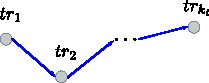
\includegraphics[width = 10cm]{./figures/img/pathproof.pdf}
\caption{车辆按照顺序接送}
\label{fig:pathproof}
\end{figure}
\par
从以上的分析中,可以知道寻找原问题的最优解,即找到最少的车辆服务所有的出行,等价于,在网络$G = (N,E)$中找到最少的路径覆盖,覆盖网络中所有的节点,并且不同的路径之间没有重合的节点。这是因为根据定理~\ref{theo:path}~,可以知道原问题所需的最少车辆数小于网络中的最少路径覆盖数,根据定理~\ref{theo:origin}~,可以知道网络中的最小路径覆盖数小于原问题中的最少车辆数。
\begin{figure}
\centering
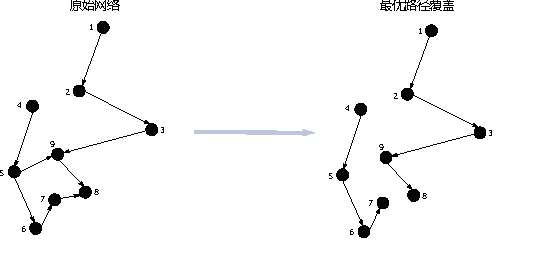
\includegraphics[width = 15cm]{./figures/img/pathcover.pdf}
\caption{在网络中找到最优路径覆盖}
\end{figure}

\subsection{将网络转化成二分网络}
在一个一般的有向网络中,我们并不能将其转换成二分网络。但是在本问题中,由于每次出行,我们都有其出发的交叉路口编号,以及达到的交叉路口的编号,我们可以通过将一个出行分为两个节点,即将出行在网络中所对应的节点,拆分为两个节点,分别代表出行的出发节点和出行的到达节点。这样所有出行的出发节点和到达节点分别组成了节点集合,这两个节点集合就是二分图中的两个节点集合,即原始的网络被转换成了一个二分网络。算法~\ref{alg:convert}~展示了上述的思路。为了更加严格说明此方法,我们将引入一些定义,定理和证明。

\begin{algorithm}[htbp]
\SetAlgoLined
\SetKwInOut{Input}{Input}\SetKwInOut{Output}{Output}
\caption{convertToBipartite($G = (N,E)$)}
\label{alg:convert}
\BlankLine
$G_b \leftarrow \emptyset$\;
$N_b \leftarrow \emptyset$\;
$E_b \leftarrow \emptyset$\;
\For{$v$ in $N$}{
  $tr_i\leftarrow$$v$所代表的出行\;
  $v_o^i\leftarrow$$tr_i$的出发交叉路口对应的节点\;
  $v_d^i\leftarrow$$tr_i$的到达交叉路口对应的节点\;
  $N_b\leftarrow N_b \cup \{v_i^o,v_i^d\}$\;
}
\For{$e = (u,v)$ in $E$}{
  $tr_i\leftarrow u$所代表的出行\;
  $tr_j\leftarrow v$所代表的出行\;
  $E_b\leftarrow E_b\cup \{(v_i^d, v_j^o)\}$\;
}
return $G_b = (N_b, E_b)$\;
\end{algorithm}

\begin{definition}[二分图]
对于图$G = (N,E)$,若$G$可以被划分成两个节点集合$S,T$,使得$S\cup T = N, S\cap T = \emptyset$,并且$\forall u, v\in S, (u,v)\notin E,(v,u) \notin E$,$\forall u, v\in T, (u,v)\notin E,(v,u) \notin E$,则$G$称为二分图。
\end{definition}
\par
图~\ref{fig:biparEx}~为一个二分图的示例。
\begin{figure}
\centering
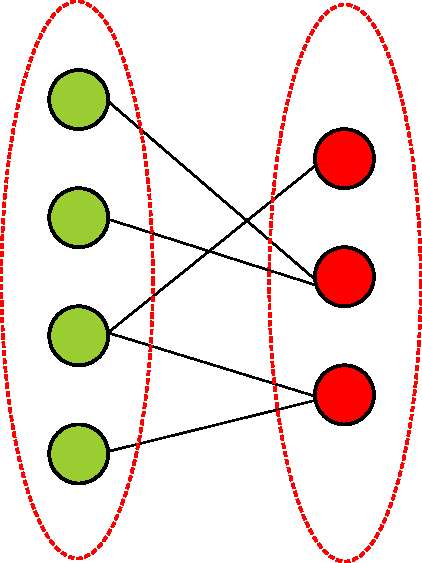
\includegraphics[width = 5cm]{./figures/img/bipartiteGraph.pdf}
\caption{二分图示例}
\label{fig:biparEx}
\end{figure}
\par
根据二分图的定义,我们可以给出如下的定理,证明我们的算法得到的图的确是二分图。
\begin{theorem}
根据算法~\ref{alg:convert}~得到的图$G_b=(N_b,E_b)$为二分图。
\end{theorem}

\begin{proof}
我们将所有出发节点组成的集合记为$N_o$,所有到达节点组成的节点组成的集合记为$N_d$,即$N_o = \{v_i^o| \forall tr_i \in Tr\},N_d = \{v_i^d| \forall tr_i \in Tr\}$,则我们证明$N_o. N_d$构成了对$G_b$的一个划分,使得$N_o\cup N_d = N_b, N_o\cap N_d = \emptyset$,并且满足二分图定义中的其他条件。
\par
首先,$N_o\cap N_d = \emptyset$是显然的,因为一个为出发节点集合,一个为到达节点集合。从算法~\ref{alg:convert}~中又可以知道$N_b$中的节点即为所有出发节点和到达节点,所以$N_o\cup N_d = N_b$。
\par
对于$E_b$中的一个边$e$,根据算法~\ref{alg:convert}~,可以将$e$记为$e = (v_i^d, v_j^o)$,而$v_i^d \in N_d, v_j^o \in N_o$。由$e$的任意性知,网络$G_b$中的所有边都满足这样的条件,所以$G_b$为二分图。
\end{proof}
\par
图~\ref{fig:bipar}~展示了将原始一般有向网络转换为二分网络。
\begin{figure}
\centering
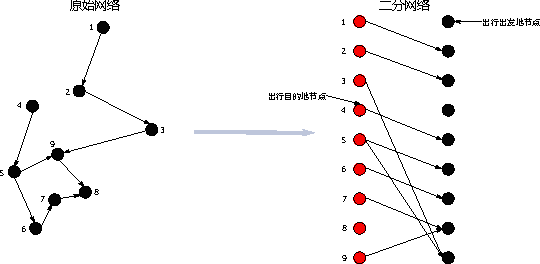
\includegraphics[height=8cm]{./figures/img/bipartiteNetwork.pdf}
\caption{將原始网络转化成二分网络}
\label{fig:bipar}
\end{figure}

\subsection{Hopcroft-Karp算法求解}
在一个一般的有向图中求解最小的路径覆盖是NP-hard的,即目前没有一个有效的多项式时间算法求解得到最优解。因此,在实际应用当中,对于交通网络而言,节点数量和边的数量都非常的大,想要求解得到最优解是几乎不可能的。但是,当有向图中没有有向圈时,存在一个高效的多项式算法求解得到最优解。无有向圈的有向图(或称为有向无环图,Directed Acyclic Network,简称DAG)的定义如下:
\begin{definition}[DAG]
一个有向图$G = (N,E)$称为是无有向圈的,如果$G$中不存在一条有向路径$P$,从$P$中一个节点$v$出发,沿着$P$的指向向前,会再次回到$v$。
\end{definition}
\par
根据以上定义,我们可以知道任何出行数据生成的有向图,都是无有向圈的,我们将其列为一个定理。
\begin{theorem}
根据全部出行数据$Tr$,以及判断两个出行是否可以被同一辆车服务的函数\texttt{isLinkable},生成的图$G = (N,E)$为DAG。
\end{theorem}
\begin{proof}
假设$P$为图$G$中的一个有向圈,并且我们可以不妨假设$P$的长度为2,因为长度为0和1的有向圈不存在,可以类似的证明长度大于2的有向圈不存在。
\par
设$P = \{(N_1, N_2), (N_2, N_1)\}$,则
\[
  t_1^d \leq t_2^o < t_2^d \leq t_1^o
\]
\par
但是,根据出行时间的意义,可以知道$t_1^d > t_1^o$,矛盾。
\par
这样我们就证明了$G$中不存在长度为2的有向圈,同样的可以证明,长度大于2的有向圈也不存在。
\end{proof}

\par
以上我们证明了,根据出行数据生成的网络为无有向圈的,因此可以在多项式时间复杂度的情形下求解最小的路径覆盖。接下来我们证明在二分图上求解最大匹配等价于在原始网络上求解最小路径覆盖。
\begin{theorem}
在$G_b = (N_b,E_b)$上的最大匹配$M$等价于在$G = (N,E)$上的最小路径覆盖。
\end{theorem}
\begin{proof}
假设$\mathcal{C} = \{P_1,\cdots, P_h\}$为$G$的最小路径覆盖,$\mathcal{M} = \{(u_1,v_1),\cdots, (u_s, v_s)\}$为$G_b$的最大匹配。
\par
由于$\mathcal{C}$为最小路径覆盖,故$h$为所有路径覆盖中最小的值。$\mathcal{C}$中共有$|N| - h$条边,为所有路径覆盖中的最大值。我们将$\mathcal{C}$中的边按照算法~\ref{alg:convert}~的方法对应到$G_b$中的边,则$\mathcal{C}$中的每一条边都对应了$G_b$中两个节点的匹配,即$\mathcal{C}$对应了$G_b$中的一个匹配,故$|\mathcal{M}| \geq |N| - h$。
\par
另一方面,对于$\mathcal{M}$中的一个匹配,两个节点分别属于不同出行,并且这两个出行满足\texttt{isLinkable}的条件,在$G$中有一条边。将$\mathcal{M}$中的匹配都对应到$G$中,则得到$G$中的一个边的集合$E^\prime$。
\par
在$E^\prime$中,没有两条边有共同的端点。否则,我们可以分两种情况讨论。
\par
两条边若有共同的到达端点,则在$G_b$中,它们对应了相同的在$N_o$中的节点,这与$\mathcal{M}$是一个匹配矛盾。
\par
两条边若有共同的出发端点,则在$G_b$中,它们对应了相同的在$N_d$中的节点,这与$\mathcal{M}$是一个匹配矛盾。
\par
所以$E^\prime$为$G$的一个路径覆盖,从而$ |\mathcal{M}|\leq N-h$。
\par
综上所述,$|\mathcal{M}| = N - h$,即求解$G$中的最小路径覆盖可以转换成求解$G_b$中的最大匹配。
\end{proof}

\par
在证明了上述结论之后,我们就可以利用在二分网络求解最大匹配的高效多项式时间算法,Hopcroft-Karp算法求解。下面我们具体介绍Hopcroft-Karp算法,为此,我们需要引入一些概念。
\begin{definition}[自由节点]
对于二分网络$G_b = (N_b, E_b)$,以及$G_b$上的一个部分匹配$\mathcal{M}$,一个节点$v\in N_b$是自由节点,如果$v$不是$\mathcal{M}$中任何一条边的端点。
\end{definition}

\begin{definition}[增广路]
对于$G_b = (N_b,E_b)$以及其上的一个部分匹配$\mathcal{M}$,一条路径$P$称为是增广路,如果$P$的起始节点为一个自由节点,并且$P$中的边为属于$\mathcal{M}$和不属于$\mathcal{M}$交替的,最后的终止节点也为一个自由节点。严格的说,$P = \{(s,v_1^1), (v_1^2, v_2^1),\cdots, (v_k^2, t)\}$,其中,$s,t$为自由节点,$v_i^1 = v_i^2, \forall i = 1,\cdots,k$,并且,当$i$为奇数时,$(v_i^2, v_{i+1}^1)\in \mathcal{M}$,$i$为偶数时,$(v_i^2, v_{i+1}^1)\notin \mathcal{M}$。
\end{definition}
\par
从以上定义中,我们可以推得$\forall i=1,2\cdots,k,v_i^1$不是自由节点,即只有$s,t$为自由节点。

\begin{theorem}
对$G_b = (N_b,E_b)$以及其上的一个部分匹配$\mathcal{M}$,$P$为$G_b$上的一个增广路,则$\mathcal{M},P$的对称差,$\mathcal{M}\oplus P$,是一个由$|\mathcal{M}|+1$个元素组成的匹配。
\end{theorem}

\begin{proof}
根据增广路的定义,设$P = \{(s,v_1^1), (v_1^2, v_2^1),\cdots, (v_k^2, t)\}$,则当$i$为奇数时,$(v_i^2, v_{i+1}^1)\in \mathcal{M}$,$i$为偶数时,$(v_i^2, v_{i+1}^1)\notin \mathcal{M}$,从而$\mathcal{M}\backslash P = \mathcal{M}\backslash \{((v_i^2, v_{i+1}^1))|i\makebox[3em]{为奇数}\}$;$P\backslash \mathcal{M} = \{(v_i^2, v_{i+1}^1)|i\makebox[3em]{为偶数}\}$。并且$|\mathcal{M}\backslash P| = |\mathcal{M}| - \frac{|P|-1}{2}, |P\backslash \mathcal{M}| = \frac{|P|+1}{2}$。所以$|\mathcal{M}\oplus P| = |\mathcal{M}|+1$。
\end{proof}
\par
由以上定理可以知道,在图中寻找增广路并且与匹配做对称差,就得到了一个严格更大的匹配。由于图中的节点和边的数量都是有限的,必定能在有限次寻找增广路之后得到最优解。Hopcroft-Karp算法的思想即是如此,不断地寻找增广路,并且与现在的部分匹配进行对称差,得到新的匹配,这个匹配是严格更大。重复此步骤,直到图中没有增广路了为止,此时的匹配就为最大的匹配,为最优解。
\par
我们将Hopcroft-Karp算法的伪代码展示如算法~\ref{alg:karp}。

\begin{algorithm}[htbp]
\SetAlgoLined
\SetKwInOut{Input}{Input}\SetKwInOut{Output}{Output}
\caption{HopcroftKarp($G_b = (N_b,E_b)$)}
\label{alg:karp}
\BlankLine
初始化匹配$\mathcal{M}\leftarrow \emptyset$\;
\While{True}{
  $\mathcal{P}\leftarrow \{P_1,P_2,\cdots, P_h\}$为图中的最大的增广路集合,并且$P_i\cap P_j=\emptyset, i\neq j$\;
  \uIf{$\mathcal{P}=\emptyset$}{
    break\;
  }
  \uElse{
    $\mathcal{M}\leftarrow \mathcal{M}\oplus (\bigcup_{i=1}^k P_i)$\;
  }
}
return $\mathcal{M}$\;
\end{algorithm}

\par
图~\ref{fig:maxMatch}~展示了Hopcroft-Karp算法的运行示意图。
\begin{figure}
\centering
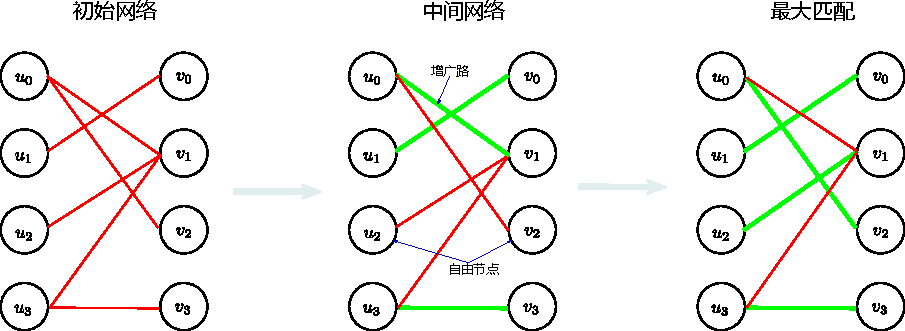
\includegraphics[width = 15cm]{./figures/img/maxMatch.pdf}
\caption{Hopcroft-Karp算法运行示意图}
\label{fig:maxMatch}
\end{figure}

\subsection{算法时间复杂度分析}
在以上的讨论中,共讨论了两个算法,一个是将原始有向图转换成二分图的算法~\ref{alg:convert}~和求解二分图中最大匹配的Hopcroft-Karp算法~\ref{alg:karp}。从算法~\ref{alg:convert}~中容易看出,主要的计算量在对每条边的循环操作,所以算法~\ref{alg:convert}~的时间复杂度为$O(|E|)$,生成的二分图的边的数量和原始图是相等的,节点的数量是原始图的两倍,即$|N_b| 2 |N|, |E_b| = |E|$。而Hopcroft-Karp算法的时间复杂度为$O(|E_b|\sqrt{|N_b|}) = O(|E|\sqrt{|N|})$。综上,这一部分的算法的总时间复杂度为$O(|E|\sqrt{|N|})$。


\section{实验结果}
我们使用在数据来源部分提到的数据进行的实际的编程计算。编程环境为Ubuntu 16.04 LTS @3.7GHz处理器,64GB RAM,编程语言为Python 3.6,使用了Numpy、Pandas、NetworkX进行数据处理,类和函数的定义编写,网络的生成和计算,使用了Multiprocessing库进行了并行计算。

\chapter{合乘情形下的最少车辆数}
\label{chap:share}
一方面,随着科学技术的发展,无人驾驶车辆正在逐渐走进人们的生活。自上世纪七十年代开始,英国、美国等国家就在无人驾驶车辆的研究生那个取得了较为瞩目的成果,而我国在2005年,第一辆城市无人驾驶汽车在上海交通大学研制成功。近些年来,随着信息技术的飞速发展,计算机视觉等领域突破性成果的出现,无人驾驶技术的研发也取得了卓越的成果。在不久的将来,我们将迎来无人驾驶车辆的市场化,彼时,路面上的无人驾驶车辆将不断地增加,有人驾驶车辆将被逐渐地取代。人们将会越来越愿意购买并使用无人驾驶车辆。
\par
无人驾驶车辆相对于有人驾驶车辆来说,可以有更多的操控性,不同的车辆之间可以更好的通过网络连接等手段传递信息,车辆的交通行为将会发生改变。无人驾驶车辆上的车载感应器,可以和智能交通系统联合工作,优化道路交叉口的车流量,交通信号灯可以更好的调度控制,改善车辆的出行效率,环节交通拥堵。同时,无人驾驶车辆的出现可以减少由于人的失误造成的交通事故。因此,对于交通领域的研究者来说,无人驾驶车辆的出现,将会带来很多可以研究的新兴问题,许多传统的问题在无人驾驶车辆的情形下也会有新的挑战。
\par
另一方面,近些年来,Airbnb和Uber等公司通过共享经济的思维把人类社会的经济模式推广到了互联网社会,通过互联网和移动设备连接了不同用户的经济行为,并且取得了很大的成功。Airbnb使得原来私人的房屋成为共享住宿服务的场所,Uber利用平台的预约功能实现车座位的共享,不同的乘客可以拼车共享。ofo,摩拜单车等公司将单车共享,使得原本私人化的单车成为临时所有物,与别人共享。这样的共享模式,使得人们可以以更低的成本得到相同的服务,同时节约了资源,减少了路面上行驶的车辆,从而进一步减少了交通拥堵,更进一步减少了尾气排放,大气污染。这样的经济模式值得推广,也给交通领域的研究者带来了许多问题可以进行研究。
\par
研究数据显示,在Uber等平台的拼车服务中,实际上每辆车的平均载客数为1.3左右,依然接近于一人一车的模式,这违反了平台提供这样的服务的初衷。因此,如何设计较为有效的算法匹配乘客和调度车辆,设计较好的平台运行机制就成为了一个重要的研究问题。本章节即是想探讨,在可以合乘的情形下,未来城市中需要多少的车辆才能服务到所有的乘客。

\section{数据来源}
我们从廊坊市,天台市,银川市,等城市采集了出租车,公交车等车辆的出行数据,包括,出行的出发地点,出发时间,到达地点,到达时间等。在数据预处理中,我们剔除了出租车和公交车等的数据,留下了私人车的出行数据,并且将出发地点和到达地点的地理位置信息都对应到了最近的交叉路口,每个城市的美俄个交叉路口都有编号,在预处理后的数据中,以编号代替交叉路口的地理位置。出发时间和到达时间都转换成秒。具体的数据解释见下表~\ref{tab:triplist}。
\begin{table}
    \centering
    \caption{出行数据的具体解释}
    \label{tab:triplist}
  \begin{tabular}{|c|p{10cm}|}
    \hline
    数据项 & 具体解释\\
    \hline \hline 
    tripRowid & 出行数据的索引,但是不是按照时间顺序排列的\\
    \hline 
    oTime & 出行的出发时间,将时间转化为秒,一天中最小的为0秒,最大的为86400秒\\
    \hline 
    dTime & 出行的到达时间,将时间转化为秒,一天中最小的为0秒,最大的为86400秒\\
    \hline 
    oInter & 出行的出发地点,将地点转化为交叉口编号,在之后的计算中出行的地理位置信息,都按照交叉口的地理信息计算\\
    \hline 
    dInter & 出行的到达地点,将地点转化为交叉口编号,在之后的计算中出行的地理位置信息,都按照交叉口的地理信息计算\\
    \hline 
  \end{tabular}
\end{table}

\par
为了计算不同出行地点之间的行驶时间,我们在将地理信息转换成最近的交叉路口信息的同时,通过百度地图API获得了不同交叉路口之间的行驶时间,生成了一个出行时间矩阵,用于之后的建模计算中。该数据表中的数据信息如表~\ref{tab:odtime}~所示。

\begin{table}
  \centering
  \caption{交叉路口之间的出行时间}
  \label{tab:odtime}
  \begin{tabular}{|c|c|}
  \hline 
  数据项 & 具体解释\\
  \hline \hline 
  o & 出发交叉口的编号\\
  \hline 
  d & 到达交叉口的编号\\
  \hline 
  time & 根据百度地图API得到的从o到d的汽车行驶时间\\
  \hline 
  \end{tabular}
\end{table}

\section{合乘判别条件}
\subsection{算法设计}
在我们的数据中,部分城市的数据,对于每个出行有其相对应的乘客数量数据,但是由于实际上,每辆车的乘客数量的平均值为1.3人,我们可以合理的假设每个出行的乘客数量都为1.因为在这里我们为了简化问题以便于讨论,我们只考虑两个出行合乘的情形,现在路面上的大部分车都为四座以上的车型,因此,假设每个出行只有一个乘客是合理的,可以满足我们讨论问题的需要。
\par
对于两个出行,如果想要通过合乘将两个出行合并为一个出行,这两个出行之间必须满足一定的时间和空间关系。
\par
时间上,首先出发的出行的到达时间必须在第二个出发的出行的出发时间之后,否则,若首先出发的出行的到达时间较早,则这两个乘客不会出现在同一辆车上,因为第一个乘客在第二个乘客出发前就可以到达自己的目的地。在数据中,我们将实际的到达时间视作为,在合乘的框架下,乘客的预计到达时间。我们希望在考虑合乘时,减少了交通拥堵,乘客的出行效率提高,所以,我们希望合乘下,每个乘客都可以在自己的预计到达时间内到达目的地。但是如果到达的太早,可能也会给乘客造成困扰。比如,如果乘客是想去电影院看电影,但是由于出行效率增加,比自己的预计到达时间提前到了半个小时。对于乘客来说,没有这半个小时或许会更好。所以,我们希望在提前到的前提下,不能提前到达太多。
\par
空间上,由于选择合乘,原本针对一个乘客规划的行车路线,需要同时再考虑另外一个乘客的出行。对于已经在车上的乘客而言,为了去接另一位乘客,可能需要偏离自己本来的行车路线,绕路到别的地方。在考虑合乘的系统框架下,乘客是接受绕路的,因为在合乘系统里,绕路是默认设定,乘客可以因为绕路而获得折扣,从而抵回损失。但是,即使这样,乘客不能接受绕路太多,因为乘客损失的时间成本不能被经济的补偿而抵回。所以,我们不允许绕路太多。对于后上车的乘客而言,如果第一位乘客的预计到达时间比第二位乘客的预计到达时间早,车辆就需要先去送第一位乘客,从而第二位乘客的路线就会绕路,同样的,我们也不允许第二位乘客绕路太多。
\par
下面,我们将严格化的说明上述想法。为此,我们分为两种情况分别讨论。
\par
在进行讨论之前,我们先引入一些记号,以使得讨论更加严格和准确。使用到的符号都列在表~\ref{tab:notation}~中。
\begin{table}
\centering
\caption{记号及其含义说明}
\label{tab:notation}
\begin{tabular}{|c|c|}
\hline 
符号 & 含义\\
\hline 
\hline
$Tr$ & 所有出行的集合 \\
\hline 
$I_i^o$ & $Tr$中的第$i$个出行$tr_i$的出发交叉路口的编号\\
\hline 
$I_i^d$ & $Tr$中的第$i$个出行$tr_i$的到达交叉路口的编号\\
\hline 
$t_i^o$ & $Tr$中的第$i$个出行$tr_i$的出发时间\\
\hline 
$t_i^d$ & $Tr$中的第$i$个出行$tr_i$的到达时间\\
\hline 
$\delta$ & 允许提前到达的时间阈值\\
\hline
$\Delta$ & 允许绕路的距离因子\\
\hline 
$\epsilon$ & 路径重合率因子\\
\hline 
\texttt{travel} & 计算行驶时间的函数\\
\hline 
\end{tabular}
\end{table}
\par
以下,以$tr_1$记为第一个出行,$tr_2$记为第二个出行。
\begin{itemize}
\item 当一个乘客的出行路线包含了另一个乘客的出行路线时,即如图~\ref{fig:cover1}~所示的情形,由于第一个出行需要在$t_1^d$之前到达,并且不可以提前太早,所以有
\begin{equation}
  t_1^d - \delta < t_1^o + travel(I_1^o,I_2^o,I_2^d,I_1^d) < t_1^d
\end{equation}
同样地,由于第二个出行也需要在$t_2^d$之前到达,并且不能提前太早,所以有
\begin{equation}
  t_2^d - \delta < t_1^o + travel(I_1^o,I_2^o,I_2^d) < t_2^d
\end{equation}
\par
对于第一个乘客而言,和二号乘客合乘之后需要绕路,但是也不能绕路太远,所以有
\begin{equation}
travel(I_1^o,I_2^o,I_2^d,I_1^d) < \Delta \times travel(I_1^o,I_1^d)
\end{equation}

      \begin{figure}
      \centering
      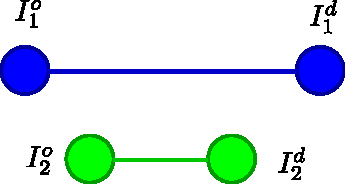
\includegraphics[width=6cm]{./figures/img/coverage1.pdf}
      \caption{第一个乘客的路线覆盖了第二个乘客的路线}
      \label{fig:cover1}
      \end{figure}

\item 当一个乘客的出行路线与另一个乘客的出行路线相交但互不包含时,即如图~\ref{fig:cover2}所示,由于第一个出行需要在$t_1^d$之前到达,并且不可以提前太早,所以有
\begin{equation}
  t_1^d - \delta < t_1^o + travel(I_1^o,I_2^o,I_1^d) < t_1^d
\end{equation}
同样地,由于第二个出行也需要在$t_2^d$之前到达,并且不能提前太早,所以有
\begin{equation}
  t_2^d - \delta < t_1^o + travel(I_1^o,I_2^o,I_1^d,I_2^d) < t_2^d
\end{equation}
\par
对于第一个乘客而言,和二号乘客合乘之后需要绕路,但是也不能绕路太远,所以有
\begin{equation}
travel(I_1^o,I_2^o,I_1^d) < \Delta \times travel(I_1^o,I_1^d)
\end{equation}
同样地,二号乘客和一号乘客合乘后,也不能绕路太远,所以有
\begin{equation}
travel(I_2^o,I_1^d,I_2^d) < \Delta \times travel(I_2^o,I_2^d)
\end{equation}
\par
同时,当在两个出行的路线重合率较低时,即在距离第一位乘客的终点较近的时候需要绕路去接第二位乘客,对于第一位乘客而言较为不公平,所以在我们的判断条件中,我们不允许,所以路径的重合率有最低的要求。
\begin{equation}
travel(I_1^o,I_2^o) < \epsilon \times travel(I_1^o, I_1^d)
\end{equation}

      \begin{figure}
      \centering
      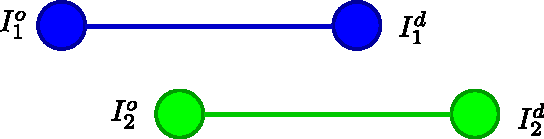
\includegraphics[width=10cm]{./figures/img/coverage2.pdf}
      \caption{第一个乘客的路线与第二个乘客的路线相交,但互不包含}
      \label{fig:cover2}
      \end{figure}
\end{itemize}

\par
将以上想法写成算法伪代码如算法~\ref{alg:isshare}~所示。
\begin{algorithm}[htbp]
\SetAlgoLined
\SetKwInOut{Input}{Input}\SetKwInOut{Output}{Output}
\caption{isShareable($tr_i,tr_j$)}
\label{alg:isshare}
\BlankLine
$tr_1,tr_2\leftarrow $为两个出行\;
\uIf{$I_i^o > I_j^o$}{
  $tr_1 \leftarrow tr_j$\;
  $tr_2 \leftarrow tr_i$\;
}
\uElse{
  $tr_1 \leftarrow tr_i$\;
  $tr_2 \leftarrow tr_j$\;
}
\uIf{$t_1^d > t_2^d$}{
  \uIf{$t_1^o + travel(I_1^o,I_2^o) < t_2^o$}{
    \uIf{($t_1^d - \delta < t_1^o + travel(I_1^o,I_2^o,I_2^d,I_1^d)$) and ($t_1^o + travel(I_1^o,I_2^o,I_2^d,I_1^d) < t_1^d$)}{
      \uIf{($t_2^d - \delta < t_1^o + travel(I_1^o,I_2^o,I_2^d)$) and ($t_1^o + travel(I_1^o,I_2^o,I_2^d) < t_2^d$)}{
        \uIf{$travel(I_1^o,I_2^o,I_2^d,I_1^d) < \Delta\times travel(I_1^o,I_1^d)$}{
          return True\;
        }
        \uElse{
          return False\;
        }
      }
    }
  }
}
\uElse{
  \uIf{($t_1^d < t_2^d$) and ($t_1^d > t_2^o$)}{
    \uIf{$t_1^o + travel(I_1^o,I_2^o) < t_2^o$}{
      \uIf{($t_1^d - \delta < t_1^o + travel(I_1^o,I_2^o,I_1^d)$) and ($t_1^o + travel(I_1^o,I_2^o,I_1^d) < t_1^d$)}{
        \uIf{($t_2^d - \delta < t_1^o + travel(I_1^o,I_2^o,I_1^d,I_2^d)$) and ($t_1^o + travel(I_1^o,I_2^o,I_1^d,I_2^d) < t_2^d$)}{
          \uIf{$travel(I_1^o,I_2^o,I_1^d) < \Delta\times travel(I_1^o,I_1^d)$}{
            \uIf{$travel(I_2^o,I_1^d,I_2^d) < \Delta\times travel(I_2^o,I_2^d)$}{
               \uIf{$travel(I_1^o,I_2^o) < \epsilon \times travel(I_1^o,I_1^d)$}{
                return True\;
              }
              \uElse{
                return False\;
              }
            }
          }
        }
      }
    }
  }
}
return False\;
\end{algorithm}

\subsection{算法时间复杂度分析}
从算法~\ref{alg:isshare}~可以知道,算法中只有\texttt{if-else}的条件判断语句和赋值语句,除了调用了\texttt{travel}函数之外,都只是加法和大小比较。并且,由于我们将交叉路口之间的行驶时间处理成了一个矩阵,并且进一步将其处理成了Hash表$Dis$,使得查询其中的一个元素的时间复杂度变为$O(1)$,所以算法总共的时间复杂度为$O(1)$。


\section{网络生成算法}
\subsection{算法设计}
上一部分,我们介绍了如何设计合理的判断两个出行是否可以合乘的条件,在时间上和空间上都加了限制,最终提出了算法~\ref{alg:isshare}~进行判断。在这一部分,我们将利用算法~\ref{alg:isshare}~进行网络的生成。
\par
每一个出行都可以视为网络上的一个节点,我们只需要对每两个节点进行判断,就可以决定它们之间是否有边相连,所以就有与算法~\ref{alg:genegraph}~类似的算法~\ref{alg:genegraphshare}。
\begin{algorithm}[htbp]
\SetAlgoLined
\SetKwInOut{Input}{Input}\SetKwInOut{Output}{Output}
\caption{generateGraph($Tr$)}
\label{alg:genegraphshare}
\BlankLine
初始化有向图网络$G \leftarrow \emptyset$\;
\For{$tr_i$ in $Tr$}{
  \tcp{$Tr(k:)$代表索引在$k$及以后的出行的集合;}
  \For{$tr_j$ in $Tr(i+1:)$}{
    \uIf{isShareable($tr_i, tr_j$)}{
      $G\leftarrow G\cup \{(tr_i, tr_j)\}$\;
    }
  }
}
return $G$\;
\end{algorithm}

\subsection{算法时间复杂度分析}
容易知道,若令$m = |Tr|$,则上述算法一共进行了$\frac{m(m-1)}{2}$次循环,每次循环中的语句,包括函数\texttt{isShareable}都是$O(1)$的,所以算法的总共的时间复杂度为$O(\frac{m(m-1)}{2})$。由于想要得到完整的网络,我们必须对$Tr$中的所有出行组成的所有出行对进行判断是否有边,由于有$m$个出行数据,我们就必须进行至少$\frac{m(m-1)}{2}$次比较。故此算法的时间复杂度只能为$O(\frac{m(m-1)}{2})$。

\section{求解所需最少车辆数}
从前两部分可以知道,生成的图以及最终生成的图都与第~\ref{cha:num}~章中类似,所以我们可以通过类似的方式,引入定义,定理和证明,说明在生成的图上寻找需要的最少车辆数和在图上寻找最大匹配时等价的。
\subsection{原问题等价于在图上寻找最大匹配}
我们希望用尽可能少的车辆服务到所有的出行,并且假定每个合乘有且仅有两个出行,所以当选择合乘的人数越多的时候,所需要的车辆就越少。这是因为,和原来的车辆数相比,一旦一名乘客合乘成功,路面上就可以减少一辆车。当减少的车辆最多时,剩下的车辆就最少。所以,直观上,在原网络中寻找最少的车辆等价于寻找最大的匹配。我们可以根据以下的定理证明。
\begin{theorem}
在原问题中求解所需最少的车辆数,等价于,在根据算法~\ref{alg:genegraphshare}~生成的图中寻找最大匹配。
\end{theorem}
\begin{proof}
设$G = (N, E)$为根据算法~\ref{alg:genegraphshare}~生成的图,$M$为$G$上的一个匹配。则想要服务到所有的乘客所需要的最少车辆数$c$为
\begin{equation}
c = |N|-2|M|+|M| = |N|-|M|
\end{equation}
所以,
\[
  \min c \Longleftrightarrow \max |M|
\]
\end{proof}

\subsection{带花树算法求解原始图上的最大匹配}
带花树算法是一个在一般图上寻找最大匹配的算法,其主要想法是在图中寻找一个有匹配边和未匹配边组成的奇圈,即花,将花进行压缩成一个点,构成新的图,在新的图上寻找增广路,以增加匹配的数量,最终得到图上的最大匹配。带花树算法的时间复杂度为$O(|N|^3)$。

\subsection{生成收缩图}
在用带花树算法进行了最大匹配的求解之后,我们可以根据求解得到的最大匹配,将匹配的出行对进行合并。因为这两个乘客选择合乘,他们都在同一辆车上,我们可以将这个组合出行看成是从最早出行的乘客的出发地点出发到最晚到达的乘客的到达地点的一次出行。所以我们可以将这两个出行所代表的图上的节点以及它们之间的边合并为一个节点。原始图根据最大匹配进行收缩后得到的收缩图的结构发生了很大的改变,我们将以两个算法分别说明如何根据匹配的结果对出行进行合并,以及如何生成收缩图。

\begin{algorithm}[htbp]
\SetAlgoLined
\SetKwInOut{Input}{Input}\SetKwInOut{Output}{Output}
\caption{combineNodes($G,\mathcal{M}$)}
\label{alg:combnode}
\BlankLine
$Tr^\prime \leftarrow \emptyset$\;
\For{$(u,v) \in \mathcal{M}$}{
  $tr_u\leftarrow $为$u$所代表的出行\;
  $tr_v\leftarrow $为$v$所代表的出行\;
  $tr_n\leftarrow $为一个新的出行\;
  $t_n^o \leftarrow \min(t_u^o,t_v^o)$\;
  $t_n^d \leftarrow \max(t_u^d,t_v^d)$\;
  $I_n^o \leftarrow I_{\argmin(t_u^o,t_v^o)}^o$\;
  $I_n^d \leftarrow I_{\argmax(t_u^o,t_v^o)}^d$\;
  $Tr^\prime \leftarrow Tr^\prime \cup \{tr_n\}$\;
}

\For{$v \in N$ and $v \notin \mathcal{M}$}{
  $Tr^\prime \leftarrow Tr^\prime \cup v$\;
}
return $Tr^\prime$\;
\end{algorithm}

\par
以上,我们根据最大匹配结果得到了合并出行后的所有出行。根据这些出行,我们再次利用\texttt{isShareable}进行判断两个出行是否可以合乘,就得到了新的图。算法如算法~\ref{alg:contract}。

\begin{algorithm}[htbp]
\SetAlgoLined
\SetKwInOut{Input}{Input}\SetKwInOut{Output}{Output}
\caption{contractedGraph($Tr^\prime$)}
\label{alg:contract}
\BlankLine
初始化无向图网络$G^\prime \leftarrow \emptyset$\;
对$Tr^\prime$中的出行按照出发时间进行排序\;
\For{$tr_i$ in $Tr^\prime$}{
  \tcp{$Tr^\prime(k:)$代表索引在$k$及以后的出行的集合;}
  \For{$tr_j$ in $Tr^\prime(i+1:)$}{
    \uIf{isShareable($tr_i, tr_j$)}{
      $G^\prime\leftarrow G^\prime\cup \{(tr_i, tr_j)\}$\;
    }
  }
}
return $G^\prime$\;
\end{algorithm}



\subsection{将无向图转换成二分图}
对于一般的无向图,我们不能将其转换成二分图,但是由于出行数据具有一定的特殊性,每条数据都包含了出行的出发地点和到达地点,我们可以将出发地点和到达地点分别视为图中的一个节点。并且,只在不同出行的到达节点和出发节点之间加无向边。由此得到的图即是二分图。算法~\ref{alg:convertshare}~展示了以上的想法。

\begin{algorithm}[htbp]
\SetAlgoLined
\SetKwInOut{Input}{Input}\SetKwInOut{Output}{Output}
\caption{convertToBipartite($G = (N,E)$)}
\label{alg:convertshare}
\BlankLine
$G_b \leftarrow \emptyset$\;
$N_b \leftarrow \emptyset$\;
$E_b \leftarrow \emptyset$\;
\For{$v$ in $N$}{
  $tr_i\leftarrow$$v$所代表的出行\;
  $v_o^i\leftarrow$$tr_i$的出发交叉路口对应的节点\;
  $v_d^i\leftarrow$$tr_i$的到达交叉路口对应的节点\;
  $N_b\leftarrow N_b \cup \{v_i^o,v_i^d\}$\;
}
\For{$e = (u,v)$ in $E$}{
  $tr_i\leftarrow u$所代表的出行\;
  $tr_j\leftarrow v$所代表的出行\;
  $E_b\leftarrow E_b\cup \{(v_i^d, v_j^o)\}$\;
}
return $G_b = (N_b, E_b)$\;
\end{algorithm}


\subsection{Hopcroft-Karp算法求解最小车辆规模}
在前面的部分,我们说明了生成出行图,并且利用带花树算法求解图上的最大匹配。图上的一个匹配即代表了一次合乘出行。我们可以将这两次出行视为一次出行,出行的出发地点即是两次出行中较早出发的乘客的出发地点,到达地点即是最后到达的乘客的到达地点。在进行了图的收缩之后,我们生成了一个基于原始图的收缩图,再利用算法~\ref{alg:convertshare}~将图转换成二分图,之后再二分图上进行求解最小车辆规模。
\par
在收缩图上求解最小车辆规模,就是求解最少的路径覆盖,使得每个出行都被服务到。图上的每个路径都代表了一辆车的先后服务,它分别服务路径上的每一个出行。求解最少的路径覆盖所有的点,就是求解最少的车辆服务所有的出行。即,二者是等价的。这由以下的两个定理保证。
\begin{theorem}\label{theo:pathshare}
对于网络$G = (N, E)$上的一个路径覆盖$\mathcal{C} = \{P_1,\cdots, P_h\}$,所有的出行都可以被服务到。
\end{theorem}

\begin{proof}
对于网络$G = (N,E)$上的一个路径$P= \{e_1 = (n_1^1, n_1^2),\cdots, e_k = (n_k^1,n_k^2)\}$,根据我们生成网络上边的算法,可以知道$n_1^1,n_1^2$(记为$tr_1,tr-2$),两个出行可以被同一辆车服务,并且,按照我们的判别条件,服务$tr_1$的车一定能在$t_2^o$之前到达$I_2^o$接到乘客。因此,出行$tr_2$的出发时间和达到时间没有延误。故和$n_1^2$有边的$n_2^2$所代表的出行不会延误,即车可以在指定时间之前到达出发地接到$n_2^2$代表的出行的乘客。以此类推,路径$P$中的所有$N(P)$个乘客都可以被同一辆车准时服务到,没有出行的延迟。因此,对于路径覆盖$\mathcal{C}$,所有的出行都可以被不同的车服务到。
\end{proof}
\par
以上我们证明了,网络$G = (N, E)$上的一个路径覆盖,如果我们以一辆车代表一个路径,则$G$上的一个路径覆盖即是可以服务所有出行的一个可行解。接下来,我们证明任意一个原问题的可行解,即一个车辆的分配使得所有出行都被服务到,都对应了$G$上的一个路径覆盖。
\begin{theorem}\label{theo:originshare}
对于所有出行的一个车辆分配,在网络$G = (N, E)$中,都存在一个路径覆盖$\mathcal{C} = \{P_1,\cdots, P_h\}$。
\end{theorem}
\begin{proof}
记$T$为所有被分配的车辆的集合,$p_t = \{tr_1,\cdots, tr_{k_t}\}, \forall t \in T$为每辆车所被分配的出行的集合,并且不失一般性的,我们假定车辆$t$即按照$tr_1,\cdots,tr_{k_t}$的顺序接送出行。则由于$tr_1,tr_2$之间满足函数\texttt{isShareable}的判别条件,所以如果将$tr_1,tr_2$都对应为网络中的一个节点,则它们之间有一条边,以此类推。所以如果将$p_t$中的所有出行都对应于网络上的节点,则$P_t = \{e_1 = (n_1^1, n_1^2),\cdots, e_{k_t} = (n_{k_t}^1, n_{k_t}^2)\}$为$G$中的一条路径,并且$P_t$中的每一个节点都代表了一个被服务的出行,其中$n_1^1$代表$tr_1$,$n_i^2, n_{i+1}^1$代表$tr_{i+1}, i = 1,\cdots, k_t$。将所有$P_t$这样的路径组合成一个路径覆盖$\mathcal{C} = \{P_1,\cdots, P_t\}$,则所有出行都在网络的节点中,所有的出行都被服务到。
\end{proof}

\par
以上我们证明了求解最小车辆规模和求解最小路径覆盖的等价性。同时,我们可以证明在收缩图上求解最小路径覆盖等价于在收缩图对应的二分图上求解最大匹配。

\begin{theorem}
在$G_b = (N_b,E_b)$上的最大匹配$M$等价于在$G = (N,E)$上的最小路径覆盖。
\end{theorem}
\begin{proof}
假设$\mathcal{C} = \{P_1,\cdots, P_h\}$为$G$的最小路径覆盖,$\mathcal{M} = \{(u_1,v_1),\cdots, (u_s, v_s)\}$为$G_b$的最大匹配。
\par
由于$\mathcal{C}$为最小路径覆盖,故$h$为所有路径覆盖中最小的值。$\mathcal{C}$中共有$|N| - h$条边,为所有路径覆盖中的最大值。我们将$\mathcal{C}$中的边按照算法~\ref{alg:convertshare}~的方法对应到$G_b$中的边,则$\mathcal{C}$中的每一条边都对应了$G_b$中两个节点的匹配,即$\mathcal{C}$对应了$G_b$中的一个匹配,故$|\mathcal{M}| \geq |N| - h$。
\par
另一方面,对于$\mathcal{M}$中的一个匹配,两个节点分别属于不同出行,并且这两个出行满足\texttt{isShareable}的条件,在$G$中有一条边。将$\mathcal{M}$中的匹配都对应到$G$中,则得到$G$中的一个边的集合$E^\prime$。
\par
在$E^\prime$中,没有两条边有共同的端点。否则,我们可以分两种情况讨论。
\par
两条边若有共同的到达端点,则在$G_b$中,它们对应了相同的在$N_o$中的节点,这与$\mathcal{M}$是一个匹配矛盾。
\par
两条边若有共同的出发端点,则在$G_b$中,它们对应了相同的在$N_d$中的节点,这与$\mathcal{M}$是一个匹配矛盾。
\par
所以$E^\prime$为$G$的一个路径覆盖,从而$ |\mathcal{M}|\leq N-h$。
\par
综上所述,$|\mathcal{M}| = N - h$,即求解$G$中的最小路径覆盖可以转换成求解$G_b$中的最大匹配。
\end{proof}

\par
同时,根据我们生成网络时的算法,以及出行数据的特殊性,我们可以证明生成的网络是有向无环图。
\begin{theorem}
根据全部出行数据$Tr^\prime$,以及判断两个出行是否可以被同一辆车服务的函数\texttt{isShareable},生成的图$G^\prime = (N^\prime,E^\prime)$为DAG。
\end{theorem}
\begin{proof}
假设$P$为图$G^\prime$中的一个有向圈,并且我们可以不妨假设$P$的长度为2,因为长度为0和1的有向圈不存在,可以类似的证明长度大于2的有向圈不存在。
\par
设$P = \{(N_1, N_2), (N_2, N_1)\}$,则
\[
  t_1^d \leq t_2^o < t_2^d \leq t_1^o
\]
\par
但是,根据出行时间的意义,可以知道$t_1^d > t_1^o$,矛盾。
\par
这样我们就证明了$G^\prime$中不存在长度为2的有向圈,同样的可以证明,长度大于2的有向圈也不存在。
\end{proof}

\par
以上我们证明了我们的网络是有向无环图,并且在对应的二分图上求解最大匹配和在图上求解最小路径覆盖是等价的。因此,我们可以利用Hopcroft-Karp算法求解。


\subsection{时间复杂度分析}
在以上的分析中,我们一共使用到了带花树算法,生成收缩图的算法,将收缩图转换成二分图的算法,以及求解最大匹配的Hopcroft-Karp算法。
\par
带花树算法的时间复杂度为$O(|N|^3)$。生成收缩图的算法共两层循环,循环的内部的时间复杂度为$O(1)$,所以算法的总时间复杂度为$O(\frac{|E|(|E|-1)}{2})$。将收缩图转换成二分图的算法含有两个循环,循环的内部的时间复杂度都为$O(1)$,一个循环的循环次数为$|N|$次,另一个循环的循环次数为$|E|$次,所以总时间复杂度为$O(|E|+|N|)$,Hopcroft-Karp算法的时间复杂度为$O(|E|\sqrt{|N|}+|N|)$。
\par
综上,本部分的所有算法的总时间复杂度为$O(|E|\sqrt{|N|}+|N|)$。
\chapter{多人合乘情境下求解乘载最多乘客}
\label{chap:ridesharing}

在上一个章节,我们考虑了两个出行合乘,并且每个出行都只有一个乘客的情形。但是,实际当中,我们可以允许很多人一起乘车,两个以上的出行进行合乘也是可行的。在现有的出租车中,车的座位数量都为4座,两个人合乘显然仍然有很多的座位被浪费,因此,在实际中,考虑多个出行进行合乘的情形也十分的必要。在上一章节中,我们为了简化问题的讨论,仅考虑了两人合乘的简单情形,在这一章节,我们将进一步讨论多个出行进行合乘的情况。也就是说,在这里,我们将不限定进行合乘的出行的数量为某一个特定的值,而是在满足车的容量限制下的大于2的任意值。例如,如果车的座位数量为4,则两个出行,三个出行,四个出行都可以进行合乘。
\par
具体来说,我们在这里要考虑的问题是:在已知车辆的位置的情况下,如何将现有的出行进行合乘,并且给合乘的出行进行车辆的分配。因为,需要已知车辆的座位数量,才可以将车辆和出行进行匹配,所以,我们需要预先知道车辆的物理信息。在进行匹配的过程中,我们需要考虑车辆和合乘后的出行的时空信息的匹配程度,所以我们也需要预先知道车辆的时空信息。在这样的情景设定下,我们考虑的目标,不再是求解最小的车辆规模,因为车辆的信息我们需要预先知道。在这里,我们考虑的目标是在给定车的数量的情况下最大化服务的乘客的数量。
% 但是实际当中,出行的乘客很多情形下都不止一个,比如一家人去火车站或者机场准备出远门,朋友们一起坐车出去看电影或者游玩,公司聚会坐车去饭店等。

\section{数学规划模型}
在这一部分,我们将利用数学规划将问题进行数学建模。在进行建模之前,我们先给出一些基本的假设。
% \subsection{基本假设}
\begin{enumerate}
\item 我们仅考虑充分短的时间段内的车辆,即,在我们考虑的时间段内,没有i虚拟的车辆到达,只有在时间开始时的车辆可供分配调度。
\item 对于每一个我们考虑的乘客,如果乘客在与他人合乘的过程中的收益大于损失,并且损失在可接受的范围内,则这位乘客将会选择合乘。
\item 对于一名车的司机而言,如果合乘时绕路的长度在他可接受的范围内,并且他的收益至少为他在不进行合乘时驾驶相同的距离和时间所得到的收益的均值,则他愿意提供合乘服务。
\end{enumerate}

\par
接下来是一些主要的记号。
\begin{longtable}{|r|l|}
        \caption{主要的记号}
            \label{tab:not}\\	
    \hline
       记号  & 含义 \\
       \endfirsthead
       记号 & 含义 \\
		\hline
		\hline
		\endhead
		\bottomrule \multicolumn{2}{r}{\textit{接下一页}} \\
		\endfoot
		\endlastfoot
       \hline
       \hline
        $\mathcal{P}$ & 乘客的全体组成的集合\\
        \hline
        $N_i$ & “邻近”(见定义~\ref{def:close})乘客$i$的左右乘客组成的集合\\
        \hline
        $\mathcal{O}$ & 出发点集合\\
        \hline
        $\mathcal{D}$ & 目的地集合\\
        \hline
        $\mathcal{DT}$ & 出发时间集合\\
        \hline
        $\mathcal{AT}$ & 最晚到达时间集合\\
        \hline
        $G_i$ & 由包含乘客$i$的两两临近的乘客组成的集合\\
        \hline
        $M_i$ & 乘客$i$可能可以合乘的出行集合\\
        \hline
        $Loss_i^m$ & 乘客$i$加入合乘$m$的损失\\
        \hline
        $\mathcal{O}_f^m$ & 合乘$m$的最终出发地点\\
        \hline
        $\mathcal{D}_f^m$ & 合乘$m$的最终到达地点\\
        \hline
        $\mathcal{DT}_f^m$ & 合乘$m$的最终出发时间\\
        \hline
        $\mathcal{AT}_f^m$ & 合乘$m$的最终到达时间\\
        \hline
        $\mathcal{M}$ & 所有的合乘组成的集合\\
        \hline
        $Dis_i^m$ & 乘客$i$加入合乘$m$所能得到的折扣\\
        \hline
        $Pay_i^m$ & 乘客$i$加入合乘$m$后应当付给司机的钱\\
        \hline
        $f_i$ & 乘客$i$在不合乘的情况下应当付的路费\\
        \hline
        $\delta$ & 在定义“邻近”中的常数距离阈值\\
        \hline
        $t$ & 在定义“邻近”中的常数时间阈值\\
        \hline
        $\Delta _m$ & 与合乘$m$匹配的司机在不提供合乘服务时,在这种情境下能够得到的收入的均值\\
        \hline
        $r_m$ & 合乘$m$中的所有乘客\\
        \hline
        $c_i^m$ & 指示变量, 当乘客$i$加入合乘$m$时为1,否则为0\\
        \hline
        $\zeta$ & 当选择合乘时,乘客所能接受的最大的损失\\
        \hline
        $\mathcal{B}$ & 可供调度的所有车辆组成的集合\\
        \hline
        $\overline{v}$ & 平均驾驶速度\\
        \hline
        $z_b^m$ & 指示变量, 当车$b$和合乘$m$匹配时为1,否则为0\\
        \hline
        $d_b^m$ & 车$b$为了接$m$所需要走过的距离\\
        \hline
        $\xi$ & 司机为了接一个合乘出行所能接受的最大的驾驶距离\\
\hline
\end{longtable}
其中,“邻近”的定义如下。
\begin{definition}[邻近]
对于乘客$i,j \in \mathcal{P}$,我们说他们是 彼此\textbf{邻近}的当且仅当$||\mathcal{O}_i - \mathcal{O}_j||_M \leq \delta $,$||\mathcal{D}_i - \mathcal{D}_j||_M \leq \delta$并且$|\mathcal{DT}_i- \mathcal{DT}_j| \leq t$,其中$||\cdot||_M$代表曼哈顿距离。
\label{def:close}
\end{definition}

\par
我们引进“邻近”的概念,是为了保证在一个合乘中的两个以及以上的乘客,在进行合乘时,不需要走很长的距离才能坐上车,或者需要等很长的时间才能等到车。当一个合乘中所有乘客都是两两邻近时,我们可以叫他们走到他们出发点的几何中心或者邻近的地方会和,一起上车。如果这样的条件不满足,则乘客可能并不会想和其他乘客一起合乘一辆车。
\[
\begin{aligned}
  \max & \sum_{b\in\mathcal{B}}\sum_{m\in\mathcal{M}} |r_m|z_b^m 
\end{aligned}
\]

\begin{align}
    s.t. \sum_{m\in M_i} c_i^m \leq&  1 \quad \forall i\in \mathcal{P}  \label{eq:c1}\\
    c_i^m =  & c_j^m \quad \forall i,j \in r_m \quad \forall m\in\mathcal{M} \label{eq:c2}\\
    \sum_{b\in\mathcal{B}}z_b^m \leq& 1 \quad \forall m\in\mathcal{M} \label{eq:c3}\\
    \sum_{m\in\mathcal{M}}z_b^m \leq& 1 \quad \forall b\in \mathcal{B} \label{eq:c4}\\
    d_b^m \leq& \xi \label{eq:c5}\\
    Loss_i^m \leq & Gain_i^m\quad \forall i\in\mathcal{P}, m \in \mathcal{M} \label{eq:c6}\\
    \Delta_m  \leq & \sum_{i\in r_m} Pay_i^m \quad \forall m \in \mathcal{M} \label{eq:c7}\\
    Loss_i^m \leq& \zeta \quad \forall i\in\mathcal{P},m\in\mathcal{M} \label{eq:c8}\\
    c_i^m, z_b^m&\in\{0,1\}\quad \forall i\in \mathcal{P}, b\in \mathcal{B}, m\in\mathcal{M} \label{eq:c9}
\end{align}

其中$Loss_i^m, Gain_i^m, Dis_i^m, f_i, \Delta_m$的定义如下:
\[
\begin{aligned}
Loss_i^m =& Function(||\mathcal{O}_i-\mathcal{O}_f^m||_M+||\mathcal{D}_i-\mathcal{D}_f^m||_M, |\mathcal{DT}_i-\mathcal{DT}_f^m|)\\
Gain_i^m = & Dis_i^m \cdot f_i\\
Dis_i^m = & Function(||\mathcal{O}_i-\mathcal{O}_f^m||_M+||\mathcal{D}_i-\mathcal{D}_f^m||_M, |\mathcal{DT}_i-\mathcal{DT}_f^m|, ||\mathcal{O}_i-\mathcal{D}_i^m||_M)\\
f_i = & Function(||\mathcal{O}_i-\mathcal{D}_i^m||_M)\\
\Delta_m = & Function(||\mathcal{O}_i-\mathcal{D}_i^m||_M,|\mathcal{DT}_f^m-\mathcal{AT}_f^m|)
\end{aligned}
\]
\par
这里,$Function$代表是函数。
\par
我们的目标函数是最大化车辆服务的乘客数量。约束\label{eq:c1}代表了,每个乘客最多只能乘一辆车,并且可能有一部分乘客没有车辆服务。约束\label{eq:c2}表示了合乘$m$的合理性。约束\label{eq:c3}和\label{eq:c4}表示了一辆车只能服务一个合乘,每个合乘只能和一辆车匹配。约束\label{eq:c5}和\label{eq:c7}保证了得到的解对司机是合理的,约束\label{eq:c6}和\label{eq:c8}保证了合乘对于合乘中每一个乘客都是合理的。约束\label{eq:c9}说明了优化问题是一个0-1整数规划问题。

\section{证明问题为NP-hard}
以下我们证明,以上我们用混合整数规划建模的问题是NP-hard的问题。我们将原问题规约为一个NP-Complete问题——Complete Coloring。
\par
从图论的语言,我们可以将Complete Coloring表述如下。
\par
\textit{给定一个图$G = (V,E)$和一个整数$k$,回答问题:是否存在一个对$V$的划分,将$V$划分为$k$或者更多的两两不交的子集合$V_1,V_2,\cdots,V_k$,使得$\forall i=1,2,\cdots,k, V_i$都是$G$上的独立集,并且$\forall i\neq j, V_i\cup V_j$不是$G$的独立集。
}
\par
在证明之前,我们先引入两个定义。
\begin{definition}[稳定对]
两个乘客$i,j\in\mathcal{P}$ are a \textbf{稳定对}当且仅当他们是互相邻近的,并且$Gain^m_i\geq Loss^m_i, Gain^m_j\geq Loss^m_j  \quad\forall m\in M_i\bigcap M_j$ 。
\end{definition}
\begin{definition}[稳定组]
一组乘客是一个\textrm{\textbf{稳定组}}当且仅当他们两两构成\textrm{稳定对}。
\end{definition}
\begin{theorem}
原问题可以规约为Complete Coloring问题,从而原问题是NP-hard的问题。
\end{theorem}
\begin{proof}
任意给定一个Complete Coloring的问题的实例,我们可以通过如下的方法构造我们的问题的一个实例。
\par
\textit{
记$P$为所有乘客的集合,乘客$p_i$为一个节点,对于每对不能形成稳定对的乘客,我们在他们的节点之间加一条边。假设对于任意的$b\in \mathcal{B}$,它可以乘载他们中的任何一个,并且车的容量足够大。
}
\par
\textit{
我们可以构建如下的映射:我们将$G$中的每一个节点$v_i$对应为$p_i\in P$的节点,并且让独立集$V_i$视为$b_i\in\mathcal{B}$中的车。我们可以观察到,可以构成稳定组的乘客可以被视为yyi一个独立集。所以有相同颜色的节点形成一个稳定组,并且与一个车匹配。车中的乘客的集合是图中的一个独立集。显然,如果我们的问题有一个解,即,存在车辆和合乘后的出行的一个匹配,则Complete Coloring问题也可解。如果存在$G$的一个满足如前所述的性质的划分,则存在一个车辆和出行匹配。
}
\end{proof}

\section{一个基于图论的精确算法}
在给出了稳定对和稳定组的定义之后,我们可以根据乘客之间的相互关系生成图。图中的每一个节点代表一个乘客,如果两个乘客之间可以合乘,我们就将他们之间加一条边。算法如算法~\ref{alg:ocnstruct}。
\begin{algorithm}[htbp]
 \SetAlgoLined
\SetKwInOut{Input}{Input}\SetKwInOut{Output}{Output}
\caption{VehicleTripGraph($G$)}
\label{alg:construct}
\BlankLine
$\mathcal{T}\leftarrow \emptyset$;$\quad$ $\mathcal{E}\leftarrow \emptyset$;\quad $\mathcal{T}_i \leftarrow \emptyset ,i=1,2,\cdots,\nu$\;

    % \For{$i$从1到$\nu$}{
    %     $\mathcal{T}_i\leftarrow \emptyset$\;
    % }
    \For{$e = (b,v)\in G$}{
        $\mathcal{T}_1\leftarrow \mathcal{T}_1\bigcup \{v\}$;\quad$\mathcal{E}\leftarrow \mathcal{E}\bigcup \{(b,v)\}$\;
    }
    \For{$\forall v_1,v_2\in \mathcal{T}_1$ and $e = (v_1,v_2)\in G$}{
        $T \leftarrow\{v_1,v_2\}$\;
        $\mathcal{T}_2\leftarrow \mathcal{T}_2\bigcup T$;\quad$\mathcal{E}\leftarrow\mathcal{E}\bigcup \{(v_1, T),(v_2,T)\}$\;
        \If{$(b,v_1),(b,v_2)\in G$}{
            $\mathcal{E}\leftarrow\mathcal{E}\bigcup \{(b,T)\}$\;
        }
    }
    \For{$j$从$3$到$\nu$}{
        \For{$\forall T_1,T_2\in \mathcal{T}_{j-1}$和$|T_1\bigcup T_2| = j$}{
            记$T_1\bigcup T_2 = \{v_1,v_2,\cdots,v_j\}$\;
            \If{$\forall k \in \{1,2,\cdots,j\}, \{v_1,v_2,\cdots,v_j\}\backslash v_k\in \mathcal{T}_{j-1}$}{
                $T\leftarrow T_1\bigcup T_2$\;
                \For{$i$从1到$j$}{
                	$\mathcal{E}\leftarrow \mathcal{E}\bigcup \{(v_i,T)\}$\;
                }
                \If{$b$可以加入$T$}{
                    $\mathcal{T}_j\leftarrow \mathcal{T}_j\bigcup T$;\quad$\mathcal{E}\leftarrow \mathcal{E}\bigcup \{(b,T)\}$\;
                }
            }
        }
    }
    $\mathcal{T}\leftarrow (\bigcup_{i\in\{1,\cdots,\nu\}}\mathcal{T}_i)\bigcup\mathcal{T}$\;
\For{每一个$b\in\mathcal{B}$}{
    \For{$t\in \mathcal{T}$}{
        \If{$b$可以与合乘$t$匹配}{
            $\mathcal{E}\leftarrow\mathcal{E}\bigcup \{(b,t)\}$
        }
    }
}
\end{algorithm}
\par
基于此算法生成的网络,我们使用动态规划的方法进行求解,我们根据动态规划提出算法~\ref{alg:optimal}。

\begin{algorithm}[htbp]
 \SetAlgoLined
\SetKwInOut{Input}{Input}\SetKwInOut{Output}{Output}
\caption{Optimal($G$)}
\label{alg:optimal}
\BlankLine
求得所有的连通分支集合$\mathcal{C}$\;
\eIf{$|\mathcal{C}| > 1$}{
    $\mathcal{W}\leftarrow \emptyset$\;
    $\mathcal{S}\leftarrow \emptyset$\;
    \For{$c\in \mathcal{C}$}{
        $w_c,s_c\leftarrow \texttt{Optimal}(G_c)$\;
        $\mathcal{W}\leftarrow\mathcal{W}+w_c $\;
        $\mathcal{S}\leftarrow\mathcal{S}\bigcup s_c $\;
    }
}{
    对$\mathcal{E}$中的所有边从$1$ 到 $n = |\mathcal{E}|$进行编号\;
    $e_1 = (u_1,v_1)\leftarrow$记为$\mathcal{E}$中的第一条边\;
    $G_1\leftarrow G$ 去除 $e_1$\;
    $G_2\leftarrow G$ 去除 $e_1,u_1,v_1$,所有$u_1$的出弧和所有$v$的入弧和它的邻居节点\;
    \For{$v\in\mathcal{V}_2$}{
        \If{$u\cap u_1 != \emptyset$}{
            删除$u$和它在中$G_2$的入弧\;
        }
    }
    $\mathcal{W}_1,\mathcal{S}_1\leftarrow \texttt{Optimal}(G_1)$;$\quad$ $\mathcal{W}_2,\mathcal{S}_2\leftarrow \texttt{Optimal}(G_2)$\;
    \eIf{$\mathcal{W}_1 > \mathcal{W}_2$}{
        return $\mathcal{W}_1, \{s_1 = 0\}\bigcup\mathcal{S}_1$\;
    }{
        return $\mathcal{W}_2, \{s_1 = 1\}\bigcup\mathcal{S}_2$\;
    }
}
\end{algorithm}

\par
为了证明我们算法的正确性,即算法的返回值和我们在上一部分提出的数学规划的解是一致的,我们将其写为一个定理。
\begin{theorem}
算法~\ref{alg:optimal}~可以返回整数规划的最优解。
\end{theorem}

\begin{proof}
首先,我们证明算法~\ref{alg:optimal}~的解满足整数规划的约束。
\begin{enumerate}
\item 当一辆车在算法执行过程中被选择了,即存在它的一条出弧$e_i\in \mathcal{E},s_i = 1$,那么它将会在之后的过程中被选择,因为它的所有出弧都在它被选择匹配之后就被删除,所以一辆车只能和一个合乘出行匹配。
\item 只要对一条边$e_i,s_i=1$,那么被匹配的出行的入弧和它的邻接节点都将从图$G$中被删除,所以一个合乘出行只能和一辆车进行匹配。
\item 当删除一个合乘出行的所有的入弧时,算法会探查到和这个出行不相容的出行,这些出行将会被算法从$G$中删除。这里的不相容是指,它们中包含相同的原始的出行。因此,每个原始的出行都在得到的解中只会出现在一个合乘出行里。
\end{enumerate}
\par
其次,我们证明算法的结果是最优的。我们利用反证法。
\par
假设有一个整数规划的最优解不能被算法~\ref{alg:optimal}~返回。假设被选择的边的编号为$e_{n_1},e_{n_2},\cdots,e_{n_k}$,即$s_{n_i}=1,\forall i\in \{1,2\cdots,k\}$将会被算法返回。那么,我们来考虑在求解过程中算法的执行过程。
\par
第一步,$s_1 = 0$或者1被选择。如果$s_1 = 0$,那么只有一条弧被删除,算法将会继续选择$s_2$的值。如果$s_2 = 0$,那么算法将会选择$s_3$的值。以此类推。当算法到达需要决定$s_{n_1}$的值的时候,0和1都是可能的选择。当$s_{n_1}=1$将会被探索时,算法将会考虑$s_{n_1+1},\cdots,s_{n_2-1}$的值。算法将$s_k=0\forall k\in \{n_1+1,\cdots,n_2-1\}$,列入算法的搜索空间中。只要算法将$s_{n_1+1},\cdots,s_{n_2-1}$赋值为0,这样的赋值就会被返回,然后算法就会选择$s_{n_2}$的值。以此类推,直到算法选择$s_{n_k}=1$,此时算法结束,因为所有的弧都被删除,这一条分支完成。
\par
从以上可以看出,赋值$s_{n_1},\cdots,s_{n_k}=1$被包含在算法的搜索空间中,因此,如果这个解是最优解并且是唯一的,算法一定会返回这个解,如果是最优的但是不是唯一的最优解,算法返回的解一定不会比这个解差,所以也是最优解。
\par
综上所述,算法返回的一定是最优解。
\end{proof}

\section{算法执行过程的一个示例}
考虑图~\ref{fig:demovtg}~中的匹配。左边红色的节点代表车辆,右边的节点代表可能的合乘。我们利用算法~\ref{alg:optimal}~求解的过程如图~\ref{fig:demo}。算法的具体执行过程如下。
\begin{itemize}
\item[第一步] 从上到下给节点编号为$1,2,\cdots,12$。
\item[第二步] 当$s_1=1$时,车$b_1$和出行1号匹配,1号出行中包含了乘客1号。
\item[第三步] 这时我们需要考虑第二辆车,如果$s_{10}=1$,则算法结束。
\item[第四步] 如果$s_{10}=0$,则算法将会考虑$s_{11}$的取值。如果$s_{11}=1$,则算法执行结束。
\item[第五步] 如果$s_{11}=0$,则算法将会考虑$s_{12}$的取值,如果$s_{12}=1$,则这条路径结束。
\item[第六步] 如果$s_{12}=1$,则此时的解不是最优解,事实上,这个解是不可行的解,因为车辆$b_2$可以乘载乘客,但是在这个解里,它并没有。
\end{itemize}
\par
算法像如上过程执行,直到所有的可能性都被发掘。最终返回的结果是使得被服务到的乘客数量最大的解。

\begin{figure}
\centering
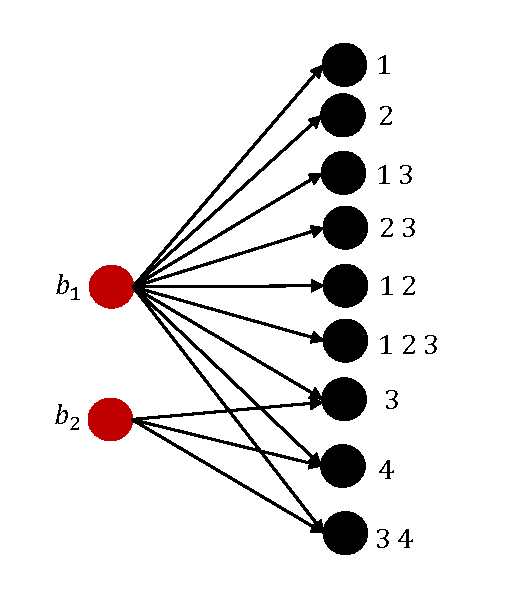
\includegraphics[width=10cm]{./figures/img/VTG.pdf}
\caption{一个示例}
\label{fig:demovtg}
\end{figure}


\begin{figure}
\centering
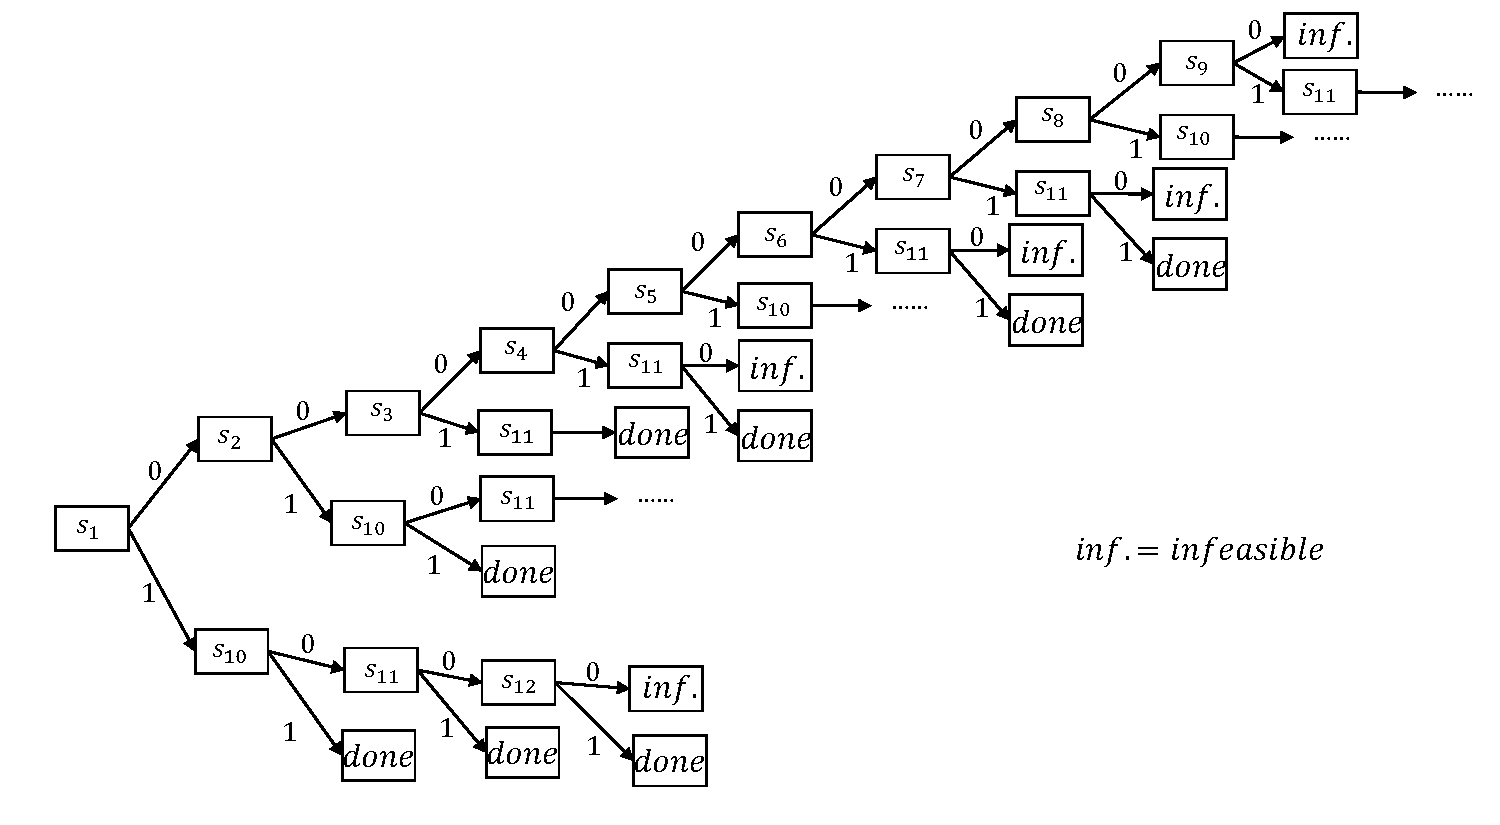
\includegraphics[width=15cm]{./figures/img/Demo_1.pdf}
\caption{算法执行过程示例}
\label{fig:demo}
\end{figure}


\section{算法时间复杂度分析}
从算法的执行过程中,我们可以得到算法~\ref{alg:optimal}~的时间复杂度的递推公式可以携程如下的形式:
\begin{equation}\label{eq:complex}
    T(|\mathcal{E^\prime}|) = T(|\mathcal{E^\prime}| - 1) + T(|\mathcal{E^\prime}| - d_b-\sum_{i = 0}^{d}d_{v_i} +d+1) + O(|\mathcal{B^\prime}|-1+|\mathcal{V^\prime}|-d-1)
\end{equation}
\par
其中$d_b,d_{v_i},d$分别代表被选择的节点的出度,入度,以及邻接节点的数量。$\mathcal{E}^\prime,\mathcal{V}^\prime,\mathcal{B}^\prime$分别代表当前边,当前出行节点,当前车辆节点。
\par
下面,求解此方程的方法展示如下。
\begin{itemize}
	\item[情形1] 当$d=0$时,即所有的合乘出行都只有一个原始出行。则问题可以被改变为最大二分匹配问题,这可以用匈牙利算法或者Hopcroft-Karp算法在多项式时间内求解。
	\item[情形2] 如果一个车辆只和形成一个稳定组的出行有边相连,则我们可以直接将车分配给该节点,这个节点包含了最多的原始出行,最多的乘客。这也可以在多项式时间内完成。
	\item[情形3] 当以上情形都不成立时,我们可以对$- d_b-\sum_{i = 0}^{d}d_{v_i} +d+1$给出一个估计。因为$d_b\geq 6, \sum_{i = 0}^{d}d_{v_i}\geq 2 (d+1),d\geq1$,那么$d_b+\sum_{i = 0}^{d}d_{v_i} -d-1\geq 8$。最差情况下,$d_b+\sum_{i = 0}^{d}d_{v_i} -d-1= 8$。在这样的情形下,为了求解原始的递推公式,我们只需要求解以下的方程:
	\begin{equation}
        x^8 = x^7 +1
    \end{equation}
    \par
    这个方程的一个实根为$x = 1.2321$。因为方程~\ref{eq:complex}~的最后一项只在现在探索的边选择为1时出现,并且在最终的解中,被选择为1的边的数量不超过车辆的数量。另外,这个附加项在一条边的$s$被指定为1时会减小,因此,附加项的时间复杂度为$O(|\mathcal{B}|^2)$。
    \par
    综上所述,算法~\ref{alg:optimal}~的时间复杂度为$O(1.2321^{|\mathcal{E}|}+|\mathcal{B}|^2)$。

\end{itemize}


\section{数据实验}
\subsection{数据来源}
本实验的数据来源于New York City Taxi \& Limousine Commission 上提供的公开数据集。数据中包含一次出行的出发地点,到达地点,出发时间,到达时间。在实验中,我们将选择不同大小的数据集以评价算法的效率。
\subsection{实验结果}
所有的实验都在Windows 10@2.20GHz,16GB RAM的笔记本电脑上完成。我们采用Python进行编程计算,采用docplex库进行求解。在不同大小的数据集上,算法的运行时间如下。
\begin{table}
\centering
\caption{实验结果}
\label{tab:exp}
\begin{tabular}{|c|c|}
\hline
边的数量 & 运行时间(s)\\
\hline
\hline
48823 & 0.89 \\
\hline
49181 & 1.39\\
\hline
60777 & 4.56\\
\hline
95215 & 8.09\\
\hline
156444 & 12.45 \\
\hline
275549 & 33.197\\
\hline
290632 & 36.86\\
\hline
514032 & 77.06\\
\hline
796878 & 198.67 \\
\hline
\end{tabular}
\end{table}
%%% 其它部分
\backmatter

%% 本科生要这几个索引,研究生不要。选择性留下。
% 插图索引
\listoffigures
% 表格索引
\listoftables
% 公式索引
\listofequations


%% 参考文献
% 注意:至少需要引用一篇参考文献,否则下面两行可能引起编译错误。
% 如果不需要参考文献,请将下面两行删除或注释掉。
\bibliographystyle{thuthesis-numeric}      % 顺序编码制
% \bibliographystyle{thuthesis-author-year}  % 著者-出版年制
\bibliographystyle{thuthesis-bachelor}     % 本科生参考文献的著录格式
\bibliography{ref/refs}


%% 致谢
% 如果使用声明扫描页,将可选参数指定为扫描后的 PDF 文件名,例如:
% \begin{acknowledgement}[scan-statement.pdf]
\begin{acknowledgement}
  衷心感谢导师李瑞敏副教授对本人的精心指导。他的言传身教将使
  我终生受益。

  在美国普渡大学西拉法叶分校土木工程系进行为期53天的暑期交流期间,承蒙Satish Ukkusuri教授热心指导与帮助,不
  胜感激。感谢 xx 实验室主任 xx 教授,以及实验室全体老师和同学们的热情帮助和支
  持!本课题承蒙国家自然科学基金资助,特此致谢。

  感谢 \LaTeX 和 \thuthesis\cite{thuthesis},帮我节省了不少时间。
\end{acknowledgement}


%% 附录
\begin{appendix}
\chapter{算法实现}
\begin{lstlisting}
def isLinkable(Trip_1, Trip_2):
    if abs(Trip_1.num - Trip_2.num) > 1:
        return False
    elif (max(Trip_1.num, Trip_2.num) == 3) and (min(Trip_1.num, Trip_2.num) == 2):
        return False
    if (Trip_1.oTime > Trip_2.oTime):
        trip_1 = Trip_2
        trip_2 = Trip_1
    else:
        trip_1 = Trip_1
        trip_2 = Trip_2
    # 这里也许可以做文章,不同的判别方式
    if trip_1.dTime < (trip_2.oTime - travelTime(trip_1.node_d,trip_2.node_o)):
        return True
    else:
        return False
\end{lstlisting}

\end{appendix}

%% 个人简历
\begin{resume}

  \resumeitem{个人简历}

  xxxx 年 xx 月 xx 日出生于 xx 省 xx 县。

  xxxx 年 9 月考入 xx 大学 xx 系 xx 专业,xxxx 年 7 月本科毕业并获得 xx 学士学位。

  xxxx 年 9 月免试进入 xx 大学 xx 系攻读 xx 学位至今。

  \researchitem{发表的学术论文} % 发表的和录用的合在一起

  % 1. 已经刊载的学术论文(本人是第一作者,或者导师为第一作者本人是第二作者)
  % \begin{publications}
  %   \item Yang Y, Ren T L, Zhang L T, et al. Miniature microphone with silicon-
  %     based ferroelectric thin films. Integrated Ferroelectrics, 2003,
  %     52:229-235. (SCI 收录, 检索号:758FZ.)
  %   \item 杨轶, 张宁欣, 任天令, 等. 硅基铁电微声学器件中薄膜残余应力的研究. 中国机
  %     械工程, 2005, 16(14):1289-1291. (EI 收录, 检索号:0534931 2907.)
  %   \item 杨轶, 张宁欣, 任天令, 等. 集成铁电器件中的关键工艺研究. 仪器仪表学报,
  %     2003, 24(S4):192-193. (EI 源刊.)
  % \end{publications}

  % 2. 尚未刊载,但已经接到正式录用函的学术论文(本人为第一作者,或者
  %    导师为第一作者本人是第二作者)。
  % \begin{publications}[before=\publicationskip,after=\publicationskip]
  %   \item Yang Y, Ren T L, Zhu Y P, et al. PMUTs for handwriting recognition. In
  %     press. (已被 Integrated Ferroelectrics 录用. SCI 源刊.)
  % \end{publications}

  % % 3. 其他学术论文。可列出除上述两种情况以外的其他学术论文,但必须是
  % %    已经刊载或者收到正式录用函的论文。
  % \begin{publications}
  %   \item Wu X M, Yang Y, Cai J, et al. Measurements of ferroelectric MEMS
  %     microphones. Integrated Ferroelectrics, 2005, 69:417-429. (SCI 收录, 检索号
  %     :896KM)
  %   \item 贾泽, 杨轶, 陈兢, 等. 用于压电和电容微麦克风的体硅腐蚀相关研究. 压电与声
  %     光, 2006, 28(1):117-119. (EI 收录, 检索号:06129773469)
  %   \item 伍晓明, 杨轶, 张宁欣, 等. 基于MEMS技术的集成铁电硅微麦克风. 中国集成电路,
  %     2003, 53:59-61.
  % \end{publications}

  % \researchitem{研究成果} % 有就写,没有就删除
  % \begin{achievements}
  %   \item 任天令, 杨轶, 朱一平, 等. 硅基铁电微声学传感器畴极化区域控制和电极连接的
  %     方法: 中国, CN1602118A. (中国专利公开号)
  %   \item Ren T L, Yang Y, Zhu Y P, et al. Piezoelectric micro acoustic sensor
  %     based on ferroelectric materials: USA, No.11/215, 102. (美国发明专利申请号)
  % \end{achievements}

\end{resume}


%% 本科生进行格式审查是需要下面这个表格,答辩可能不需要。选择性留下。
% 综合论文训练记录表
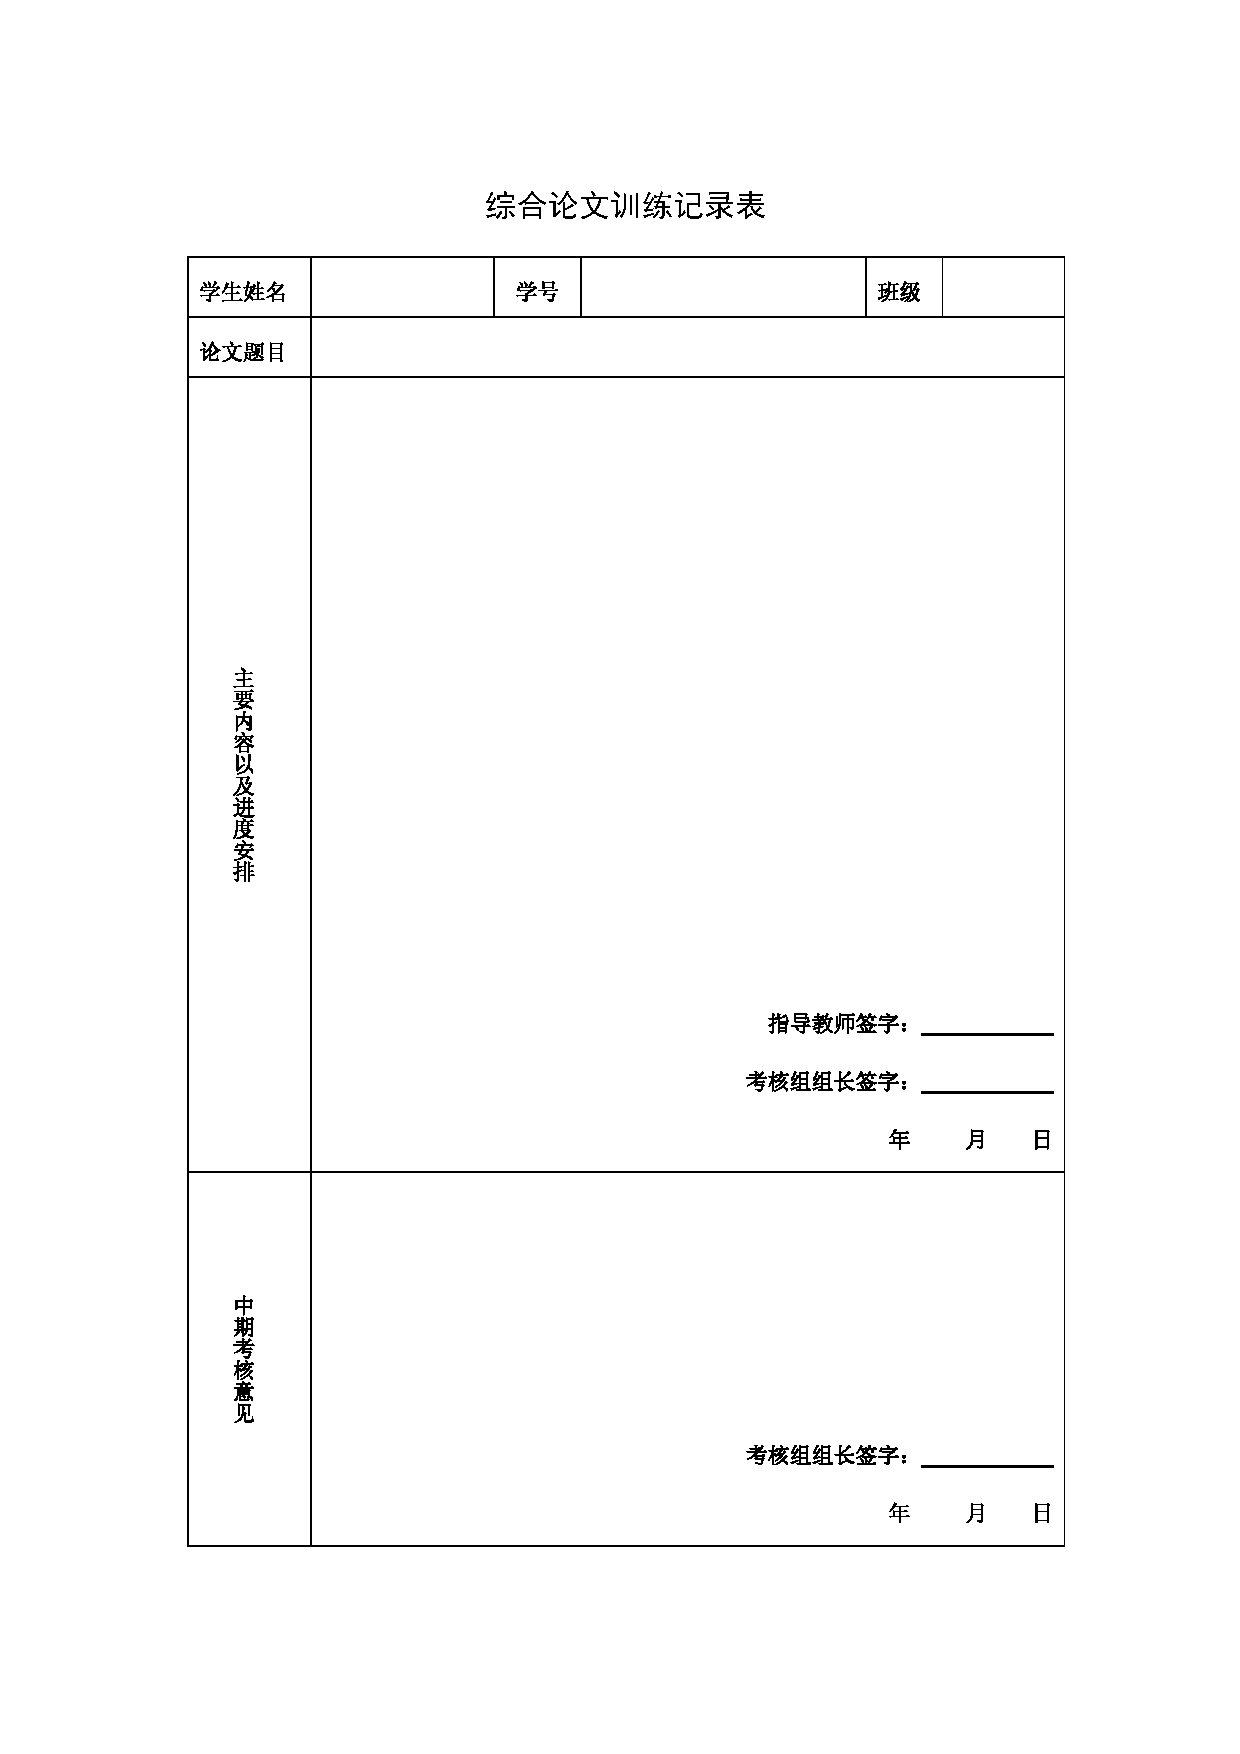
\includepdf[pages=-]{scan-record.pdf}
\end{document}
